
\documentclass{article}
\usepackage{datetime}
\usepackage{graphicx}
\usepackage{hyperref}
\usepackage{caption}
\usepackage{listings}
\usepackage[margin=1in]{geometry}
\newdate{date}{07}{10}{2019}
\renewcommand*\contentsname{Cuprins}

\begin{document}
	\begin{titlepage}
		\begin{center}
		\vspace*{1cm}
		
		\begin{center}
			\includegraphics[scale=0.6]{Source/UVTLogo}
		\end{center}

		\LARGE
		\textbf{UNIVERSITATEA DE VEST DIN TIMIȘOARA \\ FACULTATEA DE MATEMATICĂ ȘI INFORMATICĂ \\ PROGRAMUL DE STUDII DE LICENȚĂ: INFORMATICĂ ROMÂNĂ}
		\vspace{1cm}\\

		\vfill
		\Large
		\textbf{LUCRARE DE LICENȚĂ}
		\vspace{1cm}
		
		\vfill
		
		\textbf{Autor: Baș Teslim-Denis}
		\vspace{0.1cm}

		\textbf{Coordonator: Conf. Dr. Victoria Iordan}\\
		\vspace{0.1cm}		

		\end{center}
	\end{titlepage}

	\newpage

		\begin{center}
		\vspace*{1cm}

		\LARGE
		\textbf{UNIVERSITATEA DE VEST DIN TIMIȘOARA \\ FACULTATEA DE MATEMATICĂ ȘI INFORMATICĂ \\ PROGRAMUL DE STUDII DE LICENȚĂ: INFORMATICĂ ROMÂNĂ}
		\vspace{1cm}\\

		\vfill
		\Large
		\textbf{PROGRAMARE ÎN REȚEA PE DISPOZITIVE MOBILE ANDROID}
		\vspace{1cm}
		
		\vfill
		
		\textbf{Autor: Baș Teslim-Denis}
		\vspace{0.1cm}

		\textbf{Coordonator: Conf Dr. Victoria Iordan}\\
		\vspace{0.1cm}		

		\end{center}
	\newpage
		
	\Large
	\textbf{Abstract}
	\vspace{1.5cm}
	\normalsize

		This paper will present a mobile application which prioritizes efficiency, user simplicity, a new way for data to be stored and a new way for communcation between a client and the server to be held, and, respectively, ended. The application will also put into evidence the advantages of mobile programming and the advantages of mobile network programming. The mobile application will be created by using the integrated development enviorment Android Studio. This choice will allow the application to run on multiple versions of Android and will give us full acces to all of it's capabilities.\\
		This paper will also present a way of creating a server with a friendly and easy to understand User Interface by using Java's Abstract Window Toolkit ( Java AWT ), an API to develop window based applications in java. \\
		This paper will also present the use of computer network programmin which will involve writing a computer program that will enable the above said application to communicate with the server across a given network.

		
	\newpage

	\tableofcontents

 	\newpage 

	\section{Introducere}
	\vspace{1cm}
		
		Aplicația UVT Student App este o aplicație mobilă destinată studenților de la Universitatea de Vest din Timișoara.\\ 
		Aplicația va permite studentului acces la datele sale de la facultate, cum ar fi: notele pe care acesta le-a luat pe parcursul facultății (atât examene, cât și note de la laboratoare/seminare sau colocvii) precum și datele personale. Aplicația are ca scop oferirea unui acces la datele personale într-un mediu offline. \\
		
		\subsection{Motivație}
		\vspace{0.3cm}
		Atât prin utlizarea sistemului de operare mobil Android, cât și prin utilizarea serverelor create în Java cu o baza de date în SQL, aplicația UVT Student App va prezenta o modalitate ușoară și accesibilă studenților din Universitatea de Vest din Timișoara, indiferent de specializarea pe care aceștia au urmat-o, pentru a-și putea vedea informațiile strict necesare legate de facultate. \\

		Cu evoluția tehnologiei "portabile" și cu creșterea significativa a persoanelor care au un telefon mobil la îndemână, aplicațiile de tip server pot să întâmpine unele probleme în cazul în care un număr extrem de mare de utilizatori încearcă să facă o schimbare de date cu serverul respectiv ( acest lucru se poate întâmpla fie din pură coincidență, fie poate să fie un atac direct); din această cauza, serverele fie trebuie să aibe posibilitatea de a avea foarte mulți utilizatori conectați în același timp, ceea ce va duce la o investiție foarte mare de bani și de spațiu ( spre exemplu, serverele de la Google investesc aproximativ cinci sute de milioane de dolari americani doar pentru EXTINDEREA unei locații, unde acest preț nu va include serverele în sine). O metodă pentru a reduce costurile necesare pentru menținerea unui server de acest tip, o aplicație care nu necesită o conexiune constantă la internet ( ex. Youtube, Jocuri online pe telefon ) pot să folosească o metodă prin care doar datele necesare vor fi transmise, după care, conexiunea la server va fi terminată până la următoarea cerere/conexiune. În această lucrare de licență, mă voi lega de cea de a două metodă. \\ 
		
		Această metodă, în același timp, poate să fie mult mai costisitoare pentru server, deoarecere o autentificare trebuie făcută constant de către server la fiecare conexiune nouă/reînnoită. În cazul aplicației UVT Student App, această problema este evitată prin modalitatea în care această funcționează și scopul pe care aceasta îl servește. \\ \\
	
		  În această lucrare scrisă se vor prezența următoarele:
		\begin{itemize}
			\item Tehnologiile folosite pentru funcționarea corectă atât a aplicației mobile cât și a severului.
			\item Modul în care aplicația mobilă și serverul au fost create.
			\item Modul în care structurile sunt create și folosite.
			\item Detalii de implementare.
			\item Graficele UML atât a aplicației cât și a serverului.
			\item Direcțiile viitoare și aditiile noi pe care le putem adaugă atât la aplicație cât și la server.
		\end{itemize}

		\subsection{Exemplu}
		\vspace{0.3cm}
			Un exemplu deja existent și asemănător aplicației UVT Student App este site-ul "https://studentweb.uvt.ro/". Aplicația este asemănătoare site-ului, dar vine cu anumite funcționalități în plus si cu o abordare diferită.

		\subsection{Rezumat}
		\vspace{0.3cm}
		Serverul, la primirea unei conexiuni de la aplicație, va urma, de fiecare dată, 3 pași:

		\begin{itemize}

			\item 1. Verificarea email-ului primit în baza de date
			\begin{itemize}
				\item În cazul în care email-ul este găsit în baza de date, se trece la pasul 2.
				\item În cazul în care email-ul NU este găsit în baza de date, serverul va trimite, către utilizatorul aplicației, mesajul "Email sau parolă incorectă."\\
			\end{itemize}

			\item 2. Din baza de date, se va scoate parolă criptată și se va verifica cu parolă trimisă de către utilizator.
			\begin{itemize}
				\item În cazul în care parolă este corectă, se va trece la pasul 3.
				\item În cazul în care parolă NU este corectă, serverul va trimite, către utilizatorul aplicației, mesajul "Email sau parolă incorectă."
			\end{itemize}

			\item 3. În cazul în care s-a ajuns la pasul asta, știm că utilizatorul s-a identificat corect și putem să transmitem toate datele ( Datele personale + note )
			\begin{itemize}
				\item Se trimit toate datele, după care ÎNCHEIEM conexiunea.
			\end{itemize}
		\end{itemize}

	\newpage

	\section{Tehnologii folosite}
	\vspace{1cm}
		 Pentru dezvoltarea și funcționalitatea aplicației mobile UVT Student App, au fost folosite următoarele tehnologii:
	\begin{itemize}
		\item Sistemul de operare mobil Android
		\item Folosirea serverului Java
		\item SQLite, SQLiteDatabase și SQLiteOpenHelper
		\item Biblioteca RandomStringUtils
		\item Biblioteca BCryptPasswordEncoder
		\item Java SMTP
		\item Java AWT

	\end{itemize}
		\subsection{Sistemul de operare mobil Android} 
		\vspace{0.3cm}
	 Dezvoltat inițial de compania Google, urmând că după aceea să fie dezvoltat de consorțiul comerical Handset Alliance, sistemul de operare Android a fost creat pentru dispozitive și telefoane mobile, cu baza pe nucleul Linux. Sistemul de operare Android ne permite, prin intermediul bibliotecilor Java oferite și dezvoltate de către Google, permite inginerilor software scrierea de cod gestionat în limbajul Java. Android ne permite și scrierea în alte limbaje, aceastea însă trebuie compilate prin intermediul codului mașină ARM ( Advanced RISC Machine ) și nu sunt sprijinite de către Google.

	Începând cu dată de 21 Octombrie 2008, Android a fost disponibil ca Open Source. Google a decis să deschidă codul sursă pentru public ( codul era disponibil înainte doar printr-o licență Apache ). Această decizie a permis dezvoltatorilor software o modalitate de a adaugă extensii proprietare, fără a le face disponibile comunității open source. \\

	Software Development Kit-ul ( SDK ) Android-ului ne oferă un acces complet la un set de instrumente de dezvoltare. În acest SDK, ne este oferit program de depanare, biblioteci, un emulator de dispozitiv care este bazat pe QEMU, documentația necesară pentru dezvoltarea unei aplicații, mostre de cod și tutoriale. \\

		\begin{center}
			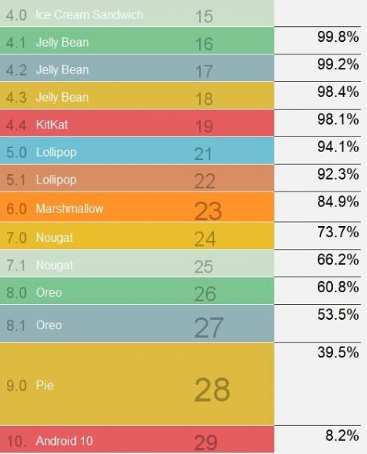
\includegraphics[scale=0.6]{Source/AndroidVersions}
		\begin{figure}[!h]
			{\caption*{Versiunile de Android curente, nivelul acestora de API și procentul de distribuție cumulativ.}}
		\end{figure}
		\end{center}

	Deși produsul Android este un produs de tip open souce, o parte din dezvoltarea software a fost continuată într-o ramură privată. \\

	Pentru folosirea si implementarea unui program nou in Android, ne vom folosi de SDK-uri si de mediul de dezvoltare Android Studio. Android Studio este bazat pe software-ul IntelliJ IDEA de la JetBrains, fiind instrumentul oficial de dezvoltare al aplicatiilor Android. \\


		\subsection {Folosirea serverului Java}
		\vspace{0.3cm}
		Pentru folosirea serverelor în Java, se va folosi biblioteca java.net . În această bibliotecă, ne sunt aduse clasele de care avem nevoie pentru implementarea aplicațiilor care se folosesc de rețele. Pentru aplicația UVT Student App, ne vom folosi de nivelul mic de API al pachetului java.net, și anume, ne vom folosi de următoarele date:
		\begin{itemize}
			\item Adrese ( identificatoare de rețea ) - folosite în întreagă librărie de java.net, adresele prezintă fie identificatorul unei gazde ce menține serverul, fie identificatorul unui client ce este conectat la capătul unui socket. 
			\item Socket-uri ( mecanism de transfer bidirecțional de date ) - folosite ca o modalitate de a stabili comunicarea între două mașini conectate printr-o rețea. În librăria java.net, ne vom folosi de două dintre cele 4 pachete oferite:
			\begin{itemize}
				\item java.net.Socket - un TCP client API, folosit pentru a face conexiunea la gazdă.
				\item java.net.ServerSocket - TCP server API, folosit pentru acceptarea conexiunilor de la clienți.
			\end{itemize}
		\end{itemize}
		Serverul este ceea ce va monitoriza conexiunile, va verifica datele primite, va putea introduce datele în baza de date și va putea transmite datele la un utilizator corect indentificat.

		\subsection {SQLite, SQLiteDatabase și SQLiteOpenHelper}
		\vspace{0.3cm}
		Pentru folosirea bazelor de date în server, se va folosi librăria java.sql . În această bibliotecă, ne este adus API-ul necesar pentru acesare și procesarea datelor ținute într-o baza de date. Acestă librărie ne va oferi acces la un cadru necesar pentru realizarea de procese.\\
		API-ul care ne este oferit este JDBC (Java DataBase Connectivity). API-ul JDBC este ceea ce ne va lasă serverul să pregătească afirmațiile pentru baza de date atât pentru introducerea datelor, cât și pentru citirea lor. \\

		 Pentru folosirea bazelor de date în aplicația mobilă, se vor folosi librăriile android.database.sqlite.SQLiteDatabase și android.database.sqlite.SQLiteOpenHelper. \\

		SQLiteDatabase este librăria care ne va permite folosirea functionalitatilor unei baze de date, precum următoarele metode:

		\begin{itemize}
			\item Create - pentru crearea unui tabel în baza de date
			\item Delete - pentru ștergerea unui tabel în baza de date
			\item Execute - pentru executarea unei comenzi în baza de date
		\end{itemize}

		În același timp, biblioteca SQLiteDatabase ne va permite rularea task-urilor comune pentru administrarea unei baze de date.\\
		
		SQLiteOpenHelper este o librărie care ne va oferi o clasa ajutatoare. Aceasta clasa ajutatoare este clasa care ne va permite crearea unor tabele in baza de date și administrarea tabelelor dintr-o baza de date. Această librărie va fi foarte importantă în aplicație, deoarece, aceasta ne va oferi o metodă de a salva datele primite de la server pe telefon astfel încât vom putea să menținem datele și după ce închidem aplicația. 

		\subsection {Biblioteca RandomStringUtils} 
		\vspace{0.3cm}
		Ne vom folosi de biblioteca org.apache.commons.lang3.RandomStringUtils pentru generarea unui șir de caractere aleator. Acest șir aleator de caractere va fi pasat către funcționalitățile bibliotecii BCryptPasswordEncoder pentru a cripta parola și pentru a o securiza într-o baza de date. Această biblioteca este sugerată la crearea unui simplu șir de caractere, care, în cazul nostru, funcționează perfect.\\ 

		Comparativ cu alte biblioteci, spre exemplu java.util.UUID.randomUUID, biblioteca RandomStringUtils, la generarea unui șir de caractere aleator, nu este exact aleator, dar, incearca sa fie cat mai apropriat. 

		\subsection {Biblioteca BCryptPasswordEncoder}
		\vspace{0.3cm}
		Ne vom folosi de biblioteca org.springframework.security.crypto.bcrypt.BCryptPassWordEncoder pentru generarea unui șir de caractere criptat. \\

Se va folosi această bibliotecă din cauza funcționalității de hashing a unei parole. Din motive de securitate într-o baza de date, abilitatea aplicației de a crea o parolă și de a hashui o parolă, după care să o stocheze într-o baza de date, este extrem de importantă, deoarece, într-un sistem normal, este imposibilă stocarea înregistrării unei parole sub formă de text simplă. \\

Din această biblioteca, ne vom folosi de clasa BCryptPasswordEncoder, o clasa ce importă PasswordEncoder, care, ne va oferi funcționalitate de a face "salt" la o parolă dată, creând astfel parolă criptată.

		\subsection{Java SMTP}

		Ne vom folosi de biblioteca java.mail și javax.mail pentru a trimite Email-uri prin folosirea aplicației web de email, Gmail. \\

Java Simple Mail Transfer Protocol este un set de linii directoare de comunicare care va permite serverului posibilitatea de a transmite un email prin intermediul internetului. Java SMTP ne va oferi posibilitatea de a schimba email-uri între un utilizator și un server, însă, pentru aplicația server, nu avem nevoie de funcționalitatea de a primi email, ci doar de a trimite. \\

Pentru trimiterea de email-uri, întâi, o să avem nevoie să creem un email. \\

După ce am creat email-ul respectiv, va trebui, însă, să activăm opțiunea de "Acces al aplicațiilor mai puțin sigure". Din păcate, acest lucru este necesar deoarece acest server nu va folosi o opțiunea de "2 factor Authentification". 

		\subsection {Java AWT}
		\vspace{0.3cm}
		Ne vom folosi de biblioteca java.awt pentru dezvoltarea unei interfețe de utilizator prin intermediul API-ului Java AWT (Abstract Window Toolkit). \\
		API-ul Java AWT este un API format din componente dependente de platforma pe care acestea au fost create. Din acest motiv, Java AWT este considerat ca fiind un API "greu", deoarece, pentru folosirea componentelor sale, acesta se folosește de sistemul de operare pe care rulează. AWT face parte din JFC ( Java Foundation Classes ), fiind unul dintre API-urile standard realizate de către Java, și aduce o interfață grafică pentru un utilizator.\\ 

		  Java AWT ne va oferi două nivele de API, însă, în această aplicație, se va folosi doar primul nivel. Acest nivel ne va oferi următoarele:
	\begin{itemize}
		\item Un set de bază de widget-uri precum:
			\begin{itemize}
				\item Butoane
				\item Cutii Text
				\item Meniuri
				\item Containere
				\item Liste
				\item Panouri
			\end{itemize}
		\item O interfață generală asemănătoare între Java și sistemul de operare pe care se lucrează. 
	\end{itemize}

	În aplicația server, ne vom folosi de următoarele widget-uri:
	\begin{itemize}
		\item{Butoane}
		\item{Panouri}
		\item{Etichete}
		\item{Câmpuri de Text}
		\item{Zonă de text}
	\end{itemize}

	 \subsubsection{Butoane}

	Butoanele vor fi folosite pentru incheiarea unei acțiuni sau pornirea unei acțiuni. 
\subsubsection*{Începerea unei acțiuni}

	Când butonul pentru începerea unei acțiuni va fi apăsat, aplicația server va deschide o nouă fereastră unde acțiunea aleasă de către utilizatorul serverului va avea loc. Această fereastră va avea, de fiecare dată, propriile widget-uri atât pentru îndrumarea utilizatorului cât și pentru salvarea datelor introduse de către utilizator. În unele cazuri, apăsarea unui buton într-o fereastră diferită de cea principala a serverului poate să creeze o fereastră în plus, necesară pentru finalizarea unei acțiuni.\\

\subsubsection*{Încheiarea unei acțiuni}

	După ce datele au fost ( sau nu ) introduse în Câmpurile de Text din interfața prezentă, aplicația va procesa datele introduse de către utilizator și va pregăti mesajul pentru baza de date. În cazul în care o anumită dată nu corespunde, aplicația va crea o eroare.\\

\subsubsection{Panouri}

	Panourile sunt folosite pentru a structura aplicația server. Aceste panouri nu sunt "vizibile" pentru utilizator, dar, sunt necesare pentru a păstra o interfață grafică consistentă și pentru a
menține toate widget-urile de o anumită categorie într-un singur loc.\\

\subsubsection{Etichete}

	Etichetele sunt folosite pentru a ajută utilizatorul. Acestea vor fi mereu însoțite de widget-uri de tipul "Câmpuri de Text" pentru a indică utilizatorului unde și ce fel de dată trebuie introdusă în câmpul de text. Aceste etichete au rol cu caracter informativ.\\

\subsubsection{Câmpuri de Text}

	Câmpurile de text sunt folosite că metodă principala de a primi informații de la utilizatorul serverului. Aceste câmpuri de text vor fi folosite pentru a pregăti mesaje pentru a fi procesate și trimise în baza de date. Aceste mesaje vor fi verificate după apăsarea unui buton și NU în timp real ( imediat după ce un câmp de text a fost completat ).\\

\subsubsection{Zonă de text}

	Zona de text se va află în interfață principala a serverului și va avea rol cu caracter informativ. Această zona de text va fi folosită de către server pentru a prezența acțiunile care au loc la nivel de server. Aceste acțiuni pot să prezinte fie când un utilizator va face orice fel de conexiune la server sau când o acțiune realizată de către utilizatorul serverul va fi încheiată cu succes. Aceste mesaje nu pot fi modificate de către utilizatorul aplicației din motive de securitate. \\

		\begin{center}
		\begin{figure}[!h]
			{\caption*{Modelul de ierarhie al claselor din Java AWT}}
		\end{figure}
			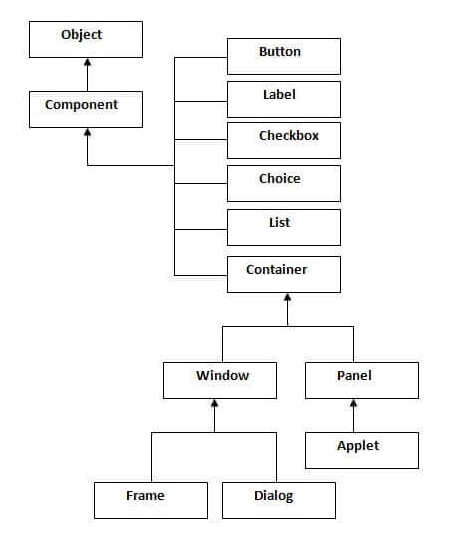
\includegraphics[scale=0.8]{Source/AWT}
		\end{center}
		\begin{center}
		\begin{figure}[!h]
			{\caption*{Exemplu de interfață grafică}}
		\end{figure}
			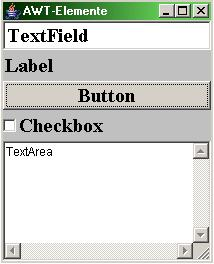
\includegraphics[scale=3.5]{Source/ExempluAWT}
		\end{center}

	\newpage	

	\section{Prezentarea detaliată a functionalităților}
	  	Acest capitol va fi despărțit în 2 subcapitole, și anume:
		\begin {itemize}
			\item Server
			\item Aplicatie
		\end{itemize}
		Se va intra în detaliu foarte meticulos asupra celor 2 subcapitole și se vor prezenta toate detaliile legate de acestea și toate funcționalitățile lor.
		\subsection{Server}
			\subsubsection{Prezentare generală}

			Serverul va fi rulat pe sistemul de operare Windows 10 folosind sistemul de construire și al administrare al proiectelor, Maven.\\

			Funcționalitățile principale care fac parte de interfață serverului sunt următoarele:
		\begin{itemize}
			\item Cine se conectează în timp real la server.
			\item Funcționalitatea de a adauga un student nou în baza de date.
			\item Funcționalitatea de a adauga o notă unui student în baza de date.
		\end{itemize}

		Se va intra în detaliu asupra fiecărei categorii de mai sus în subsubcapitoelele de mai jos.

	\begin{center}
		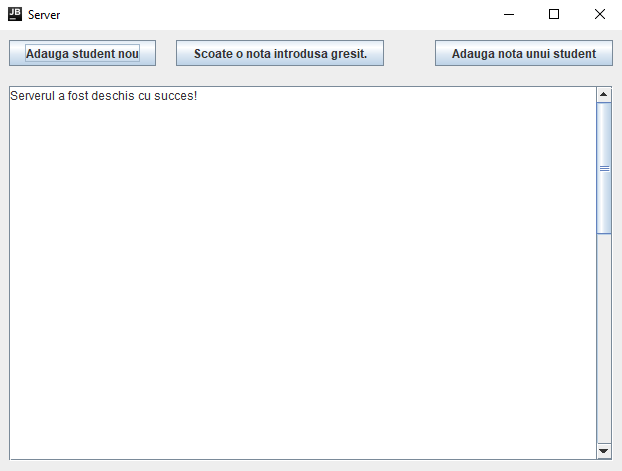
\includegraphics[scale=0.7]{Source/Server}
		\begin{figure}[!h]
			{\caption*{Interfață serverului.}}
		\end{figure}
	\end{center}

			\subsubsection{Inițializare server}

			 În primul rând, pentru funcționalitatea corectă unui server care poate fi accesat din orice locație cu o rețea validă, va trebui, pe computerul gazdă care va ține serverul, să "deschidem" un port. \\

			Porturile sunt o parte integrantă a modelului de comunicare al internetului. Porturile sunt canalele prin care aplicațiile pot să comunice cu aplicațiile software de pe un computer server. Un port deschis, în ciuda numelui său, nu ne prezintă doar dacă se poate ajunge la un port, ci, ne spune dacă o aplicație software ascultă momentan acel port sau nu. \\

			Pentru deschiderea unui port, va trebui să accesăm adresa de IP al routerului nostru. Pentru a face asta, vom accesa IP-ul 192.168.1.1 . O dată cu accesarea acestui IP, ni se va oferi următoarea interfață.

	\begin{center}
		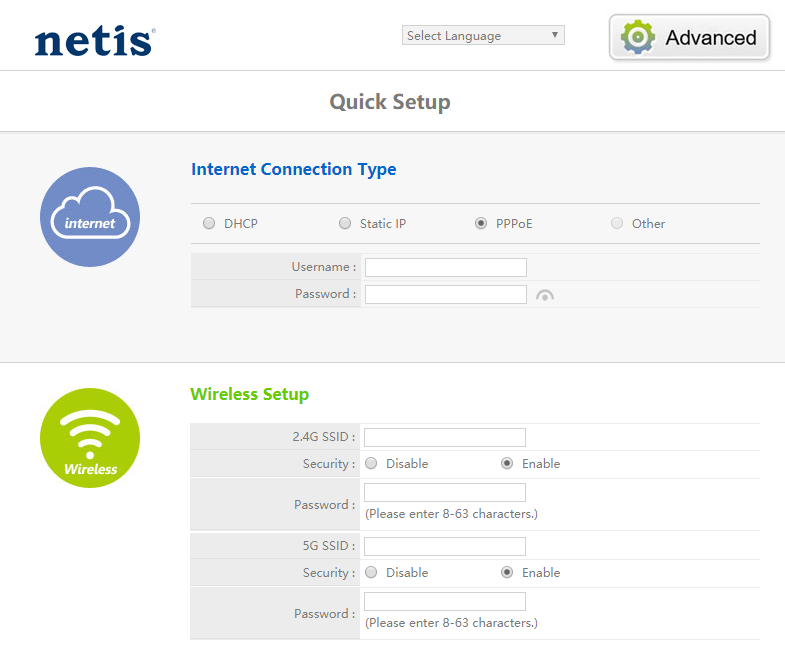
\includegraphics[scale=0.5]{Source/Router}
		\begin{figure}[!h]
			{\caption*{Exemplu interfață Router (NETIS)}}
		\end{figure}
	\end{center}

			În interfață respectivă, ne vom duce la butonul de Advanced. De acolo, ne vom duce în continuare la opțiunea de forwarding, unde, pentru a deschide un port prin care vom putea comunica cu aplicațiile din afara rețelei locale, vom alege portul prin care se va putea face comunicarea. Un exemplu de cum ar trebui să arate un port deschis se află în figura [\ref{PortDeschisEx}].

	\begin{center}
		\begin{figure}[!h]
			{\caption*{Exemplu port deschis.}}
		\end{figure}
		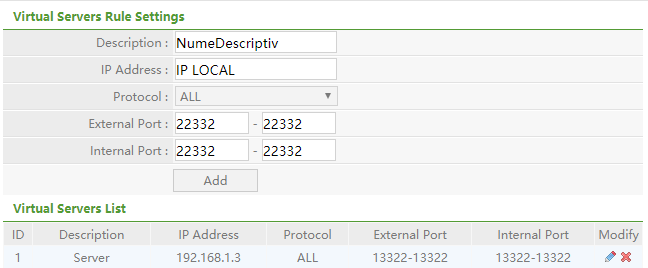
\includegraphics[scale=0.7]{Source/PortOpened}
	\end{center}\label{PortDeschisEx}
		
	După ce portul a fost deschis, aplicația de server poate să fie setată pe portul respectiv. \\
	După deschiderea serverului, vom inițializa o metodă prin care vom putea să începem să ascultăm mesajele de pe portul respectiv.\\

	\begin{verbatim}
	private static ServerSocket serversocket;
private static Socket socket;	
	private static BufferedReader bufferedreader;
		.
		.
		.
	  serversocket = new ServerSocket( Port );
	  socket = serversocket.accept();
	  bufferedreader = new BufferedReader( 
		  new InputStreamReader( socket.getInputStream()) );
	\end{verbatim}

		  Serverul, începând de acum, va putea să primească mesajele care vor veni pe portul respectiv.

			\subsubsection{Funcționalitatea de a arăta ce se întâmplă în timp real}
		Interfața serverului ne va prezenta. într-un mod ușor de citit, mesajele produse în timp real de către server. \\
		Mesajele care pot apărea în cutia text de producție a serverului sunt de 2 feluri:
	\begin{itemize}
		\item Mesaje create de la comunicare dintre server și aplicație
		\item Mesaje create de către server la introducerea anumitor date noi în baza de date.
	\end{itemize}

	\begin{center}
		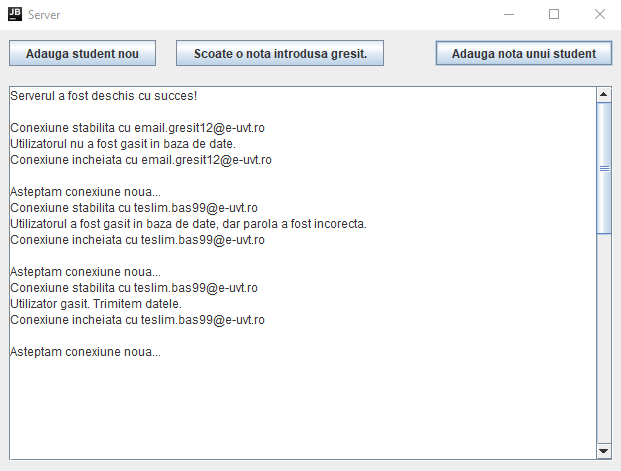
\includegraphics[scale=0.7]{Source/ServerOutput}
		\begin{figure}[!h]
			{\caption*{Exemplu mesaje transmise în server.}}
		\end{figure}
	\end{center}
	
	\subsubsection{Funcționalitatea de a adaugă un student nou}\label{Adauga Student}

		Funcționalitatea de a adăuga un student nou în baza de date este una dintre cele două funcționalități principale ale serverului. Odată la apăsarea butonului, aplicația server va deschide o fereastră nouă în care se va permite introducerea anumitor date pentru inserarea unui student. \\

	 	În această ferestra, se vor prezenta următoarele date, care, trebuiesc obligatoriu completate:
	\begin{itemize}
		\item Nume Student
		\item Prenume Student
		\item Dată Naștere ( DD/MM/YYYY )
		\item Cetățenie Student
		\item CNP Student
		\item Email de rezerva
		\item Specializare \\
	\end{itemize}

	\begin{center}
		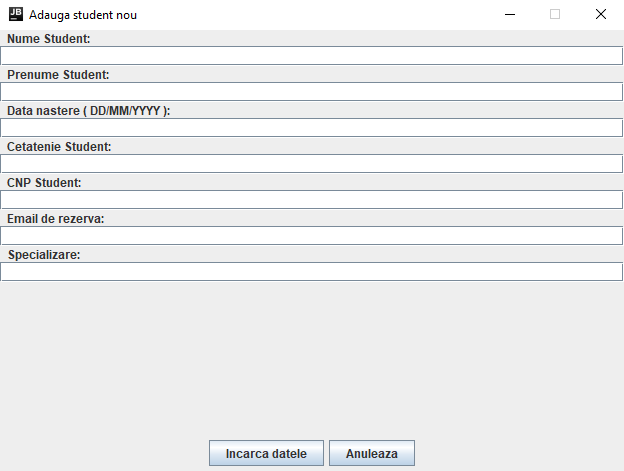
\includegraphics[scale=0.8]{Source/StudentNou}
		\begin{figure}[!h]
			{\caption*{Interfața de introducere a unui student nou.}}
		\end{figure}
	\end{center}

		\subsection*{Verificări Generale}
		În primul rând, se va verifica lungimea fiecărui câmp. În cazul în care lungimea câmpului este egală cu zero, utilizatorul care introduce datele, odată cu apăsarea butonului "Submite", va fi promptat cu fereastră "Introducere eronată a datelor". Această fereastră va păstra mereu același titlu în cazul unei erori, dar, conținutul ferestrei va fi mereu diferit pentru fiecare eroare detectată. În cazul în care mai multe erori sunt găsite la o introducere eronată a datelor, se va arată doar prima eroare găsită. Un exemplu de introducere eroanata a datelor la CNP este arătată în imaginea următoare.

	\begin{center}
		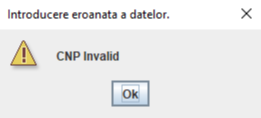
\includegraphics[scale=1]{Source/StudentNouEroare}
		\begin{figure}[!h]
			{\caption*{Exemplu de eroare la introducerea unui student.}}
		\end{figure}
	\end{center}
	
		În cazul în care lungimea unui câmp este egală cu zero, conținutul ferestrei va fi înlocuit cu "Toate câmpurile sunt obligatorii!". \\

		În al doilea rând, se va verifica introducerea corectă a caracterelor introduse. Introducerea corectă a caracterlor introduse va verifică, spre exemplu, dacă în câmpul "CNP" sunt introduse doar numere și NU litere. Alt exemplu ar fi pentru câmpul "Nume Student", unde, acesta, trebuie să conțină doar litere și nu cifre sau caractere speciale ( spațiul este permis ).

		\subsection*{Nume Student și Prenume Student}
		
		Câmpurile "Nume Student" și "Prenume Student" vor fi în aceeași categorie deoarece se fac aceleași verificări, aceste verificări fiind cele generale menționate mai sus. În cazul în care
în câmpurile "Nume Student" sau "Prenume Student" sunt găsite caractere speciale sau numere, utilizatorul va fi promptat cu fereastra de "Introducere eronată a datelor", unde, conținutului erorii va fi "Numele poate conține doar litere.", respectiv "Prenumele poate conține doar litere."

		\subsection*{Dată Naștere}

		Formatul acceptat în câmpul "Dată Naștere" va fi ZZ/LL/AAAA, unde:
		\begin{itemize}
			\item ZZ - Ziua
			\item LL - Luna
			\item AAAA - Anul
		\end{itemize}		

		Înainte de verificările care sunt făcute pentru datele datei de naștere a studentului, în cazul în care cele 2 verificări generale nu vor întoarce o eroare, ziua, luna și anul de naștere vor fi puse în 3 variabile care vor fi folosite mai târziu pentru CNP.  

		\subsubsection*{Anul}
		 Anul introdus de către utilizator nu va putea să fie mai mare decât Anul Curent - 10 și Anul Curent - 80. Spre exemplu, dacă aplicația este utilizată în anul 2020 pentru a introduce un student născut în 1964, aplicația nu va produce erori ( asta în cazul în care restul datelor sunt corecte ), dar, în cazul în care studentul introdus este născut în anul 2011 sau în anul 1939, aplicația va întoarce eroarea "Dată de naștere invalida.".
		
		\subsubsection*{Luna}
		Luna introdusă de către utilizator nu va putea să fie mai mare de cât 12 sau mai mică de cât 1, dar, poate să fie egală. Lunile sunt la fel ca și cele din calendar ( 1 - Ianuarie, 2 - Februarie, 3 - Martie..., 12 - Decembrie ).

		\subsubsection*{Ziua}
		Ziua introdusă de utilizator va fi situațională, fiind dependenda de luna și de an. \\

		Dacă ziua este egală cu 31, se va verifica luna introdusă de către utilizator. În cazul în care luna în care studentul este născut este egală cu o luna în care data de 31 este existentă, ( 1,3,5,7,8,10,12 ), serverul nu va returna nici o eroare. În cazul în care luna în care studentul este născut NU este egală cu o luna în care data de 31 este existentă, serverul va întoarce eroarea "Dată de naștere invalida.".

		Dacă luna este egală cu 02 ( Februarie ), o verificare adițională va fi necesară în cazul în care ziua este egală cu 29 (în cazul în care ziua este egală cu 30/31 iar luna este 02, serverul va produce automat o eroare). Aceste verificare va consta în verificarea anului pentru a se determina dacă este bisect. Această verificare va fi făcută în felul următor:

	\begin{verbatim}
   	 public boolean VerificaAn(int year)
    	{
       	 	if ( year % 4 == 0 )
       		{
            		if ( year % 100 == 0 )
            		{
               			 if ( year % 400 == 0 )
                		{
                    			return true;
                 } else return false;
            		}else return true;
        	}
       		return false;
    	}
	\end{verbatim}

		\subsection*{Cetatenie Student}

		Verificările făcute în câmpul "Cetățenie Student" sunt doar verificările generale. În cazul în care în câmpul "Cetățenie Student" se vor găsit caractere speciale sau numere, utilizatorul va fi promptat cu fereastră de "Introducere eroanata a datelor", unde, conținutul erorii va fi "Cetățenia poate continue doar litere.".

		\subsection*{CNP}
		În cazul verificărior făcute câmpului "CNP Student", lungimea câmpului va trebui, obligatoriu, să fie de exact 13 cifre. În cazul în care acest lucru nu este îndeplinit, aplicația va întoarce eroarea "Introducere eronată a datelor" cu descrierea "CNP Invalid.". \\

		În primul rând, se va verifica dacă dată de naștere este valida cu CNP-ul. Se va verifică dacă Ziua, Luna și Anul nașterii ( ultimele 2 cifre din An ) corespund cu datele din CNP. Spre exemplu, o persoană născută în 01/04/1996 va trebui să conțînă în CNP, obligatoriu, datele următoare: 960401.

	\begin{verbatim}
        if ( !ZiuaNastere.equals( CNP.substring(5,7)) )
           {
           	return Error = "CNP-ul nu corespunde cu data de nastere";
       	   }
        if ( !LunaNastere.equals(CNP.substring(3,5)) )
           {
            	return Error = "CNP-ul nu corespunde cu data de nastere";
           }
        if ( !AnNastere.substring(2).equals(CNP.substring(1,3)) )
           {
            	return Error = "CNP-ul nu corespunde cu data de nastere";
           }
	\end{verbatim}

		În al doilea rând, se va verifică CIFRA DE CONTROL a CNP-ului. Cifra de control a CNP-ului este un cod autodetector aflat în relație cu toate celalte 12 cifre ale CNP-ului. Cifra de control va fi calculată prin următoarea metodă: fiecare cifra din CNP va fi luată și înmulțită cu cifra de pe aceeași poziție din numărul 279146358279. Rezultatele obinute vor fi însumate, astfel încât, finalul este împărțit cu rest la 11. În cazul în care restul obținut este 10, atunci, cifra de control va fi 1.

	\begin{verbatim}
        String[] CNPBuilder = CNP.split("");
        int[] SumaCNP = new int[CNP.length()];
        for (int i=0; i<CNP.length(); i++)
        {
            SumaCNP[i] = Integer.parseInt(CNPBuilder[i]);
        }
	        suma = SumaCNP[0]*2 + SumaCNP[1]*7 + SumaCNP[2]*9 + SumaCNP[3]*1 + SumaCNP[4]*4 
                + SumaCNP[5]*6 + SumaCNP[6]*3 + SumaCNP[7]*5 + SumaCNP[8]*8
                + SumaCNP[9]*2 + SumaCNP[10]*7 + SumaCNP[11]*9;

        suma%=11;
        if (suma==10)
        {
            suma = 1;
        }
	\end{verbatim}

	În cazul în care Cifra de Control nu va corespunde cu cea din CNP, utilizatorul va fi promptat cu eroarea "Introducere eronată a datelor" care va avea descrierea "CNP Invalid.".
		\subsection*{Email de rezervă}

	Verificările făcute în câmpul "Email rezervă" sunt doar verificările generale. În cazul în care în câmpul "Email de rezervă" NU se vor gasi caracterele speciale "@" si ".", utilizatorul va fi promptat cu fereastră de "Introducere eroanata a datelor", unde, conținutul erorii va fi "Email Invalid.".

		\subsection*{Specializare}

		Verificările făcute în câmpul "Specializare" sunt doar verificările generale. În cazul în care în câmpul "Cetățenie Student" se vor găsit caractere speciale sau numere, utilizatorul va fi promptat cu fereastră de "Introducere eroanata a datelor", unde, conținutul erorii va fi "Specializarea poate continue doar litere.". 

		\subsection*{Pregătirea Datelor}
		După ce toate verificările au fost făcute, iar nici o eroare nu a fost semnalată, serverul va trece la etapa de pregătire a datelor în sistem.\\

		\subsubsection*{Creare Email}
		Pentru a stoca detaliile studentului în baza de date, va trebui, mai întâi, să creem Email-ul studentului.\\
		Email-ul studentului va fi format din primul șir de caractere din prenume + "." + primul șir de caractere din nume + ultimele două cifre din anul nașterii (spre exemplu, anul 1999 va avea ultimele două cifre 99). Aceste date se vor pune într-un singur șir de caractere, la finalul căruia se va adaugă șirul de caractere "@e-uvt.ro". \\
		
		Emailul studentului va trebui să fie unic în baza de date și creat după detaliile studentului (Nume, Prenume, An). Pentru a obține acest lucru, se va lua noul email creat și se va caută în baza de date printr-o funcție recursivă. În cazul în care acesta nu există în baza de date, nici o modificare nu va avea loc. În cazul în care acesta EXISTĂ în baza de date, se va adaugă, începând de la unu, la începutul email-ului, numărul de repetiții al acestui email.

	\begin{verbatim}
    public String CreateEmail(String Nume, String Prenume, String An)
    {
        String Email = "";

        String[] BuildMessageNume = Nume.toLowerCase().split(" ", 2);
        String[] BuildMessagePrenume = Prenume.toLowerCase().split(" ", 2);

        Email += BuildMessagePrenume[0];
        Email += ".";
        Email += BuildMessageNume[0];
        Email += An.substring(2);
        Email += "@e-uvt.ro";

        return Email;
    }
	\end{verbatim}

		\subsubsection*{Creare Parola}
		
		După ce crearea Email-ului a fost reușită, va trebui să fie creată o parolă pentru a stoca detaliile studentului în baza de date. \\

		În primul rând, va trebui să creem o parolă nouă. Acest lucru va fi făcut prin generarea unui șir de caractere aleator de 6 cifre. Acest sir de caractere de șase cifre va fi ales din șirul de caractere următor: "abcdefghijklmnopqrstuvwxyz0123456789". După ce șase caractere aleatoare au fost alese din acest șir de caractere, parolă va fi criptată de către biblioteca BCryptPasswordEncoder [\ref{PasswordEncoder}]. 
		
	\begin{verbatim}
    public String CreatePassword()
    {
        String PasswordChars = "abcdefghijklmnopqrstuvwxyz0123456789";
        BCryptPasswordEncoder passwordEncoder = new BCryptPasswordEncoder();
        String parola = RandomStringUtils.random( 6, PasswordChars );

        return passwordEncoder.encode(parola);
    }
	\end{verbatim}

		\subsection*{Introducerea datelor}
		După ce toate verificările au fost făcute, Email-ul și Parolă au fost create iar nici o eroare nu a fost semnalată, serverul va trece la etapă de introducere a datelor în sistem.\\

		Pentru a introduce datele în sistem, serverul va trebui mai întâi să creeze o conexiune la baza de date. Pentru a crea o conexiune la baza de date, prin folosirea librăriei SQL [\ref{SQL}], vom crea o funcție de conectare la server.

	\begin{verbatim}
    public Connection SqlConnect()
    {
        Connection connection = null;

        try {
            Class.forName("org.sqlite.JDBC");
            connection = DriverManager.getConnection("jdbc:sqlite:CALE_BAZA_DE_DATE");
            connection.setAutoCommit(false);
        } catch (Exception e) {
            System.out.println(e.getClass().getName() + ". " + e.getMessage());
        }

        return connection;
    }
	\end{verbatim}\label{Conectare}

		După ce conexiunea a fost creată, vom pregăti un mesaj de tipul \textbf{PreparedStatement} . Acest tip de mesaj ne va permite încărcarea sigură a datelor în baza de date. Siguranță această este necesare în cazul în care, un utilizator va încarcă, fie din greșeală sau din intenție, un student cu una dintre date egală cu \textbf{DROP TABLE "NUME TABEL"}. 

	\begin{center}
		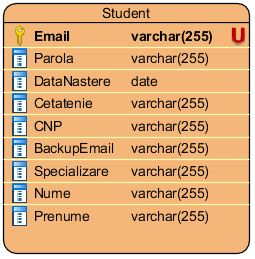
\includegraphics[scale=0.6]{Source/Student}\label{Student}
		\begin{figure}[!h]
			{\caption*{Model al tabelului Student.}}
		\end{figure}
	\end{center}

		După ce toate verificările de mai sus au fost făcute, conexiunea la baza de date a fost creată și mesajul a fost pregătit către baza de date, se vor încarcă datele în baza de date și vom primi un mesaj de succes în interfață principala a serverului. Se vor introduce datele in baza de date prin următorul mesaj SQL: 
	\begin{verbatim}
		INSERT INTO Student(Email, Parola, DataNastere, Cetatenie, CNP, 
                     BackupEmail, Specializare, Nume, Prenume) VALUES (?,?,?,?,?,?,?,?,?)
	\end{verbatim}
 
		După ce datele au fost introduse în baza de date, aplicația se va folosi de biblioteca SMTP ( Simple Mail Transfer Protocol ) [\ref{SMTP}]pentru a trimite un email cu credențialele noului utilizator. Recipientul acestui email la care se vor trimite aceste date este email-ul de rezervă introdus de către utilizatorul serverului. \\
		  Email-ul care va trimite aceste mesaje este "uvtstudentapp@gmail.com". Acest email a fost creat \textbf{pentru uz PERSONAL și din motive de utilizare a unei aplicații personale}.\\
		În primul rând, pentru a trimite un email, serverul va trebui să se conecteze la email-ul care va trimite mesajul. Pentru aceasta, ne vom folosi de biblioteca java.util.Properties . Folosind această biblioteca, putem să ne conectăm la portul 587 de la serverele GMAIL pentru a ne autentifica. În cazul în care o autentificare nu se va putea realiza, serverul ne va anunța în interfața sa principală. \\
		
	\begin{verbatim}
        Properties properties = new Properties();
        properties.put("mail.smtp.host", "smtp.gmail.com");
        properties.put("mail.smtp.port", "587");
        properties.put("mail.smtp.auth", "true");
        properties.put("mail.smtp.starttls.enable", "true");

        Authenticator auth = new Authenticator() {
            @Override
            protected PasswordAuthentication getPasswordAuthentication() {
                return new PasswordAuthentication(fromEmail, password);
                }
        };

	\end{verbatim}
		
		  După ce o autentificare a fost realizată iar nici o eroare nu a fost ridicată de către server sau primită de la serverele GMAIL, serverul va trimite mesajul recipientului.

	\begin{center}
		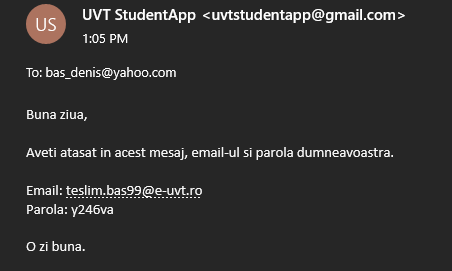
\includegraphics[scale=0.8]{Source/ExempluMail}
		\begin{figure}[!h]
			{\caption*{Exemplu Email primit.}}
		\end{figure}
	\end{center}

			\subsubsection{Funcționalitatea de a adaugă o notă unui student}

	Funcționalitatea de a adaugă o notă unui student este o altă funcționalitate principala a serverului. Odată cu apăsarea butonului, aplicația server va deschide o fereastră nouă în care se va permite introducerea anumitor date pentru inserarea unei note pentru un anumit student. \\

	\begin{center}
		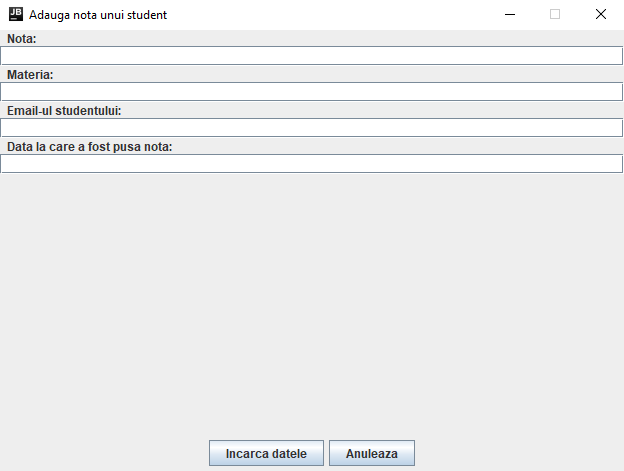
\includegraphics[scale=0.8]{Source/ServerNota}
		\begin{figure}[!h]
			{\caption*{Interfața de introducere a notelor.}}
		\end{figure}
	\end{center}

	În această ferestra, se vor prezenta următoarele date, care, trebuiesc obligatoriu completate:
	\begin{itemize}
		\item Nota
		\item Materia
		\item Email-ul studentului
		\item Data la care a fost pusă nota
	\end{itemize}

	Vom trece prin fiecare dată de intrare de mai sus și se va intra în detaliu asupra verificărilor care au loc la introducerea unui note pentru un student.

		\subsubsection*{Verificări Generale}
		În primul rând, se va verifica lungimea fiecărui câmp. În cazul în care lungimea câmpului este egală cu zero, utilizatorul care introduce datele va, odată cu apăsarea butonului "Submite", va fi promptat cu fereastră "Introducere eronată a datelor". Această fereastră va păstra mereu același titlu în cazul unei erori, dar, conținutul ferestrei va fi mereu diferit pentru fiecare eroare detectată. În cazul în care mai multe erori sunt găsite la o introducere eronată a datelor, se va arată doar prima eroare găsită. Un exemplu de introducere eroanata a datelor la Notă este arătată în imaginea următoare.
	
	\begin{center}
		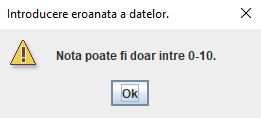
\includegraphics[scale=1]{Source/ServerNotaEroare}
		\begin{figure}[!h]
			{\caption*{Interfața serverului.}}
		\end{figure}
	\end{center}

		\subsubsection*{Nota}

	Câmpul "Notă", pe lângă verificările generale, va verifică dacă notă care este introdusă este între zero și zece. În cazul în care notă NU se va cuprinde între zero și zece, utilizatorul va fi promtat cu fereastră de "Introducere eronată a datelor", unde, conținutul erorii va fi "Notă poate fi dolar între 0-10.".\\
	Câmpul "Notă" poate acceptă note de tip \textbf{double} (spre exemplu, 5.6, 7.2, 9.9 ).

		\subsubsection*{Materie}

	Campul "Materie", pe langa verificarile generale, va verifica daca materia introdusa de catre utilizator exista in baza de date (Acest lucru poate fi modificat), in tabelul Materie. Acest lucru, va fi facut prin cautarea Materiei in baza de date, realizat, din nou, prin functia de conectare mentionata mai sus si printr-un mesaj de tipul \textbf{PreparedStatement}.

	\begin{center}
		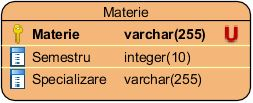
\includegraphics[scale=0.7]{Source/Materie}
		\begin{figure}[!h]
			{\caption*{Model al tabelului Materie.}}
		\end{figure}
	\end{center}

	\begin{verbatim}
	SELECT * FROM Materie WHERE Materie=?
	\end{verbatim}

	În cazul în care Materia NU este găsită în baza de date, utilizatorul va fi promtat cu fereastra de "Introducere eronată a datelor", unde, conținutul erorii va fi "Materia nu a fost găsită în baza de date.". 

		\subsubsection*{Email-ul studentului}

	Câmpul "Email-ul studentului", pe lângă verificările generale, va verifică dacă email-ul introdus de către utilizator există în baza de date, în tabelul Student menționat mai sus [\ref{Student}]. Acest lucru, va fi făcut prin căutarea Email-ului în baza de date, realizat, din nou, prin funcția de conectare menționată mai sus [\ref{Conectare}] și printr-un mesaj de tipul \textbf{PreparedStatement}.

	\begin{verbatim}
	SELECT * FROM Student WHERE Email=?
	\end{verbatim}

		În cazul în care Email-ul NU este găsit în baza de date, utilizatorul va fi promtat cu fereastra de "Introducere eronată a datelor", unde, conținutul erorii va fi "Nu s-a gasit email-ul in baza de date.". 
		\subsubsection*{Data la care a fost pusă nota}
	
	Câmpul "Dată", pe lângă verificările generale, va verifică dacă data introdusa este una valida. Aceasta validitate va verifica urmatoarele:
	\begin{itemize}
  		\item Dată să nu fie mai mare de cât data curentă.
		\item Notă trecută să fie în anul curent sau în anul anterior.
		\item În cazul în care ziua este 29 și luna este Februarie, se va verifică dacă anul este bisect.
	\end{itemize}
	
		În cazul în care Anul nu va corespunde cu verificarea de mai sus, utilizatorul va fi promptat cu fereastra de "Introducere eronată a datelor", unde, conținutul erorii va fi "Anul poate să fie doar cel curent sau cel anterior". \\

		În cazul în care Dată nu va corespunde cu restul verificărilor, utilizatorul va fi promptat cu fereastra de "Introducere eronată a datelor", unde, conținutul erorii va fi "Dată introdusă nu este valida".

		\subsubsection{Funcționalitatea de a șterge o notă care a fost introdusă greșit}

	Funcționalitatea de a scoate o notă care a fost introdusă greșit este o alta functionalitate principala a serverului. Această funcționalitate va fi folosită în cazul în care, din neatenție, un utilizator al serverului va introduce o notă greșită unui student.\\

	Această fereastră va prezenta o singură dată, care, trebuie obligatoriu completată.: Email-ul studentului.

	\begin{center}
		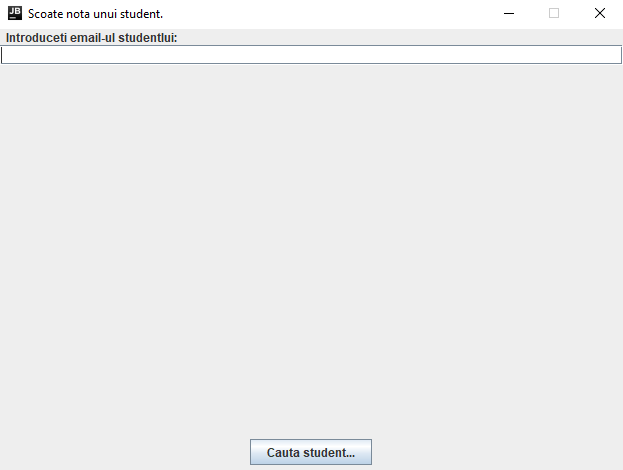
\includegraphics[scale=0.5]{Source/ServerScoate}
		\begin{figure}[!h]
			{\caption*{Interfața de eliminare a unei note.}}
		\end{figure}
	\end{center}

	\subsubsection*{Email-ul Studentului}
		  Câmpul "Email-ul studentului" va verifica, printr-o căutare în baza de date, dacă Email-ul studentului există. \\

		În cazul în care studentul NU este găsit în baza de date, utilizatorul serverului va fi promptat cu fereastra de "Introducere eronată a datelor", unde, conținutul erorii va fi "Studentul nu există în baza de date.".
	
	\begin{center}
		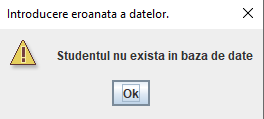
\includegraphics[scale=0.8]{Source/ServerScoateEroare}
		\begin{figure}[!h]
			{\caption*{Exemplu eroare la căutarea studentului.}}
		\end{figure}
	\end{center}

		În cazul în care studentul există în baza de date, dar, din anumite motive ( spre exemplu, dacă studentul a fost introdus recent în baza de date) studentul NU are note în baza de date, utilizatorul serverului va fi promptat cu fereastra de "Introducere eronată a datelor", unde, conținutul erorii va fi "Studentul nu există în baza de date.".

	\begin{center}
		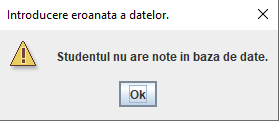
\includegraphics[scale=0.8]{Source/ServerScoateEroare1}
		\begin{figure}[!h]
			{\caption*{Exemplu de eroare la găsirea notelor unui student.}}
		\end{figure}
	\end{center}

		În cazul în care studentul există în baza de date, iar cel puțin o singură notă poate fi găsită în baza de date, aplicația server ne va prompta o ferestra nouă. În această fereastră, se vor afișa toate notele studentului, în ordinea în care acestea au fost puse în catalog ( Ordonate după data din baza de date ).\\

	\begin{center}
		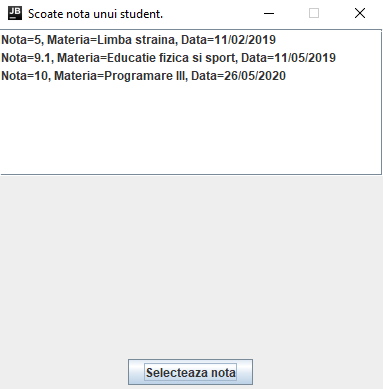
\includegraphics[scale=0.8]{Source/ServerScoateLista}
		\begin{figure}[!h]
			{\caption*{Exemplu cu lista notelor unui student.}}
		\end{figure}
	\end{center}

		Pentru noua fereastră, utilizatorul serverului va putea să vadă toate notele studentului respectiv și va avea opțiunea de selectare a uneia dintre acestea. După ce o selecție a fost făcută, utilizatorul serverului va avea opțiunea de apăsarea butonului "Selectează notă". \\

		Acest lucru este obținut astfel:
\begin{verbatim}
    String SQLStatement = "SELECT Note.Nota, Note.Materie, Note.Student, Note.Date 
        FROM Note WHERE Note.Student=? ORDER BY Note.Date";
   .
   .
   .
        try (Connection connection = this.SqlConnect();
             PreparedStatement preparedStatement = connection.prepareStatement(SQLStatement)) {
            preparedStatement.setString(1, Email);
            ResultSet resultSet = preparedStatement.executeQuery();

            while (resultSet.next()) {
                String Nota = resultSet.getString("Nota");
                String Materie = resultSet.getString("Materie");
                String Data = resultSet.getString("Date");

                builder.append(Nota);
                builder.append("=");
                builder.append(Materie);
                builder.append("=");
                builder.append(Data);
                builder.append("~");
            }

        } catch (SQLException e) {
            System.out.println("A aparut o eroare in baza de date..");
        }
\end{verbatim}

		În cazul în care nici o selecție nu va fi făcută, iar butonul "Selectează notă" va fi apăsat, utilizatorul serverului va fi promptat cu fereastră de "Introducere eronată a datelor", unde, conținutul erorii va fi "Nu ați făcut nici o selecție".

	\begin{center}
		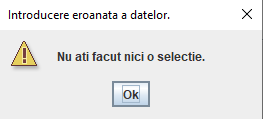
\includegraphics[scale=0.8]{Source/ServerScoateEroare2}
		\begin{figure}[!h]
			{\caption*{Exemplu de eroare la selectarea unei note.}}
		\end{figure}
	\end{center}

		După ce o selecție a fost făcută, iar utilizatorul serverului va apasă butonul "Selectează notă", utilizatorul va mai fi promptat, încă o ultima dată, cu o fereastră unde va fi întrebat dacă este sigur de opțiunea dorită.\\

	\begin{center}
		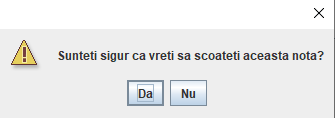
\includegraphics[scale=0.8]{Source/ServerScoateListaPrompt}
		\begin{figure}[!h]
			{\caption*{Exemplu de avertizare dupa apăsarea butonului "Selectează notă".}}
		\end{figure}
	\end{center}

		În cazul în care utilizatorul serverului va apăsa pe butonul "Nu", fereastră nouă deschisă se va închide și o nouă alegere va fi posibilă de făcut.\\

		În cazul în care utilizatorul serverului va apăsa pe butonul "Da", fereastră nouă deschisă se va închide alături de fereastră cu notele afișate, după care, aplicația va scoate din baza de date notă respectivă.  \\

		Acest lucru este obținut astfel:
	\begin{verbatim}
    String SQLStatement = "DELETE FROM Note WHERE Nota=? AND Materie=? AND Student=? AND Date=?";
    .
    .   
    .
    try (Connection connection = this.SqlConnect();
             PreparedStatement preparedStatement = connection.prepareStatement(SQLStatement))
        {
            preparedStatement.setString(1, Nota[1]);
            preparedStatement.setString(2, Materie[1]);
            preparedStatement.setString(3, NumeStudent);
            preparedStatement.setString(4, Data[1]);

            preparedStatement.executeUpdate();
            connection.commit();

            return true;
        } catch (SQLException e) {
            System.out.println("A aparut o eroare in sistem.");
        }
    
	\end{verbatim}
		\subsection{Aplicatia UVT Student App}

			\subsubsection{Funcționalitatea de verificare a unei conexiuni la internet}

		Odată cu pornirea aplicației, la nivel local, se va verifica, în primul rând, dacă există o conexiune valabilă la internet. Acest lucru se va face cu ajutorul librăriei android.net.ConnectivityManager [\ref{ConnMan}]. O conexiune la o rețea Wi-Fi sau o conexiune la o rețea mobilă este considerată o rețea valida. Aplicația NU va verifica dacă o conexiune Wi-Fi poate accesa o rețea MAN ( Metropolitan Area Network ).\\

		Verificarea se va face astfel: 
		\begin{verbatim}
    public boolean CheckForInternetConnection() {
        ConnectivityManager ConnectManag = (ConnectivityManager) getSystemService
            (Context.CONNECTIVITY_SERVICE);
        if (ConnectManag.getNetworkInfo(ConnectivityManager.TYPE_MOBILE).getState() 
              == NetworkInfo.State.CONNECTED ||
        ConnectManag.getNetworkInfo(ConnectivityManager.TYPE_WIFI).getState() 
              == NetworkInfo.State.CONNECTED) {
            return true;
        }
        return false;
    }
		\end{verbatim}

	În cazul în care o conexiune nu este valabilă ( Funcția va întoarce fals ), aplicația va crea un mesaj de tipul \textbf{TOAST} pentru a informa utilizator. Mesajul va utilizatorul: "Nu există o rețea mobilă disponibilă."

	\begin{center}
		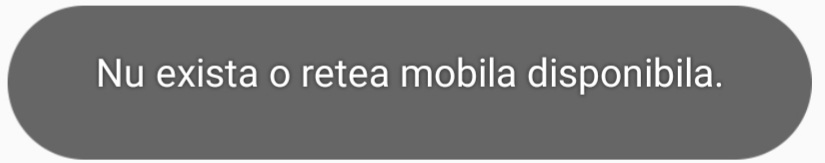
\includegraphics[scale=0.25]{Source/AplicatieRetea}
		\begin{figure}[!h]
			{\caption*{Exemplu de mesaj informativ (Rețea indisponibilă).}}
		\end{figure}
	\end{center}

	Dacă aplicația mobilă este pornită fără a avea o conexiune valida la internet și mesajul "Nu există o rețea mobilă disponibilă" este afișat, pornirea unei conexiuni la rețeaua mobilă este valida și posibilă de către aplicație.

			\subsubsection{Funcționalitatea de Login}

 	 Funcționalitatea de Login a aplicației mobile va avea două verificări:
	\begin{itemize}
		\item O verificare locală a datelor.
		\item O verificare la nivel de server a datelor.
	\end{itemize}

		\subsubsection*{Verificarea locală a datelor}
		Aceasta verificare se va face din doua motive. \\
		Aplicatia este nevoita sa se asigure daca datele trimise de catre utilizator sunt conform standardelor cerute de catre server. Standardele cerute de catre server pentru credentialele utilizatorului sunt urmtoarele:
	\begin{itemize}
		\item Email-ul trimis să conțină caracterul "@".
		\item Email-ul trimis să conțină șirul de caractere "e-uvt.ro".
		\item Email-ul trimis să conțină cifre ( corespunzător anului de naștere ).
  		\item Parolă trimisă de către utilizator aibe cel puțin 6 caractere ( Acest lucru este poate fi modificat într-o versiune mai nouă a aplicației).
	\end{itemize} \label{Credentiale}

		În cazul în care aceste date pe care utilizatorul dorește să le trimită nu corespund cu standardele de mai sus, aplicația NU va realiza o conexiune cu serverul. Acest lucru este făcut pentru a reduce costurile serverului, după care, utilizatorul va fi promptat cu un mesaj de tipul \textbf{TOAST}, unde, conținutul mesajului va fi "Email sau parolă invalidă". \\

	\begin{center}
		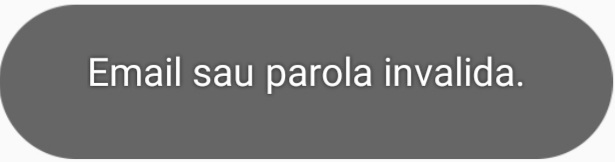
\includegraphics[scale=0.25]{Source/AplicatieEmailINVALID}
		\begin{figure}[!h]
			{\caption*{Exemplu de mesaj eronat informativ (Email sau parolă invalidă).}}
		\end{figure}
	\end{center}

		În cazul în care aceste date pe care utilizatorul dorește să le trimită corespund cu standardele de mai sus și aplicația are o conexiune la internet, aplicația va trece la următorul pas (Verificarea la nivel de server a datelor).

		\subsubsection*{Verificarea la nivel de server a datelor}
	După ce verificările locale au fost făcute și o conexiune valida a fost găsită, aplicația va trimite datele către server. \\

	În primul rând, serverul va caută email-ul utilizatorului în baza de date. Acest lucru se va face printr-un simplu mesaj SQL pentru a verifică existența lui:

	\begin{verbatim}
	SELECT * FROM Student WHERE Email=?
	\end{verbatim}
	
		În cazul în care studentul NU este găsit în baza de date, aplicația va trimite utilizatorului mesajul "Email sau parolă greșită.", dar, în server, mesajul care va fi afișat va fi "Utilizatorul nu a fost găsit în baza de date.". Cum acest lucru nu poate fi observat de către utilizatorul aplicației, putem afișa în server motivul exact care a provocat această eroare. Nu vom spune utilizatorului aplicației dacă doar Email-ul sau doar Parolă au fost greșite din motive de securitate.\\

		În cazul în care studentul este găsit în baza de date, se va trece la a două etapă. \\

	În al doilea rând, serverul, după ce a găsit Email-ul studentului în baza de date, va returna parola din baza de date. Această parolă, prin utilizarea bibliotecii BCryptPasswordEncoder, [\ref{PasswordEncoder}]
va lua ca prim parametru parolă trimisă de către utilizator și o va compara cu cel de-al doilea parametru, aceasta fiind parolă Hash-uită din baza de date.

		În cazul în care parolă trimisă de către utilizatorul aplicației NU va corespunde cu parolă din baza de date, serverul va trimite utilizatorului "Email sau parolă greșită.", dar, în server, mesajul care va fi afișat va fi "Utilizatorul a fost găsit în baza de date, dar parolă a fost incorectă." Cum acest lucru nu poate fi observat de către utilizatorul aplicației, putem afișa în server motivul exact care a provocat această eroare. Nu vom spune utilizatorului aplicației dacă doar Email-ul sau doar Parolă au fost greșite din motive de securitate. \\

		După ce serverul a trimis către, aplicația mobilă mesajul "Email sau parolă greșită.", aplicația va crea un mesaj de tip \textbf{TOAST} cu conținutul mesajului respectiv.

	\begin{center}
		\includegraphics[scale=0.25]{Source/AplicatieEmailGresit}
		\begin{figure}[!h]
			{\caption*{Exemplu de răspuns de la server. (Email sau parolă invalidă)}}
		\end{figure}
	\end{center}

	\begin{center}
		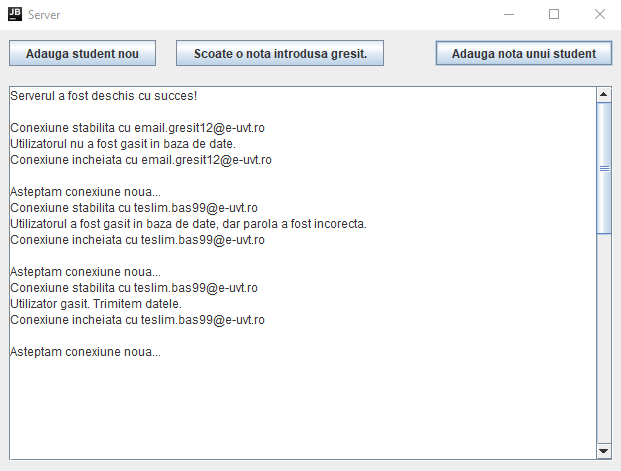
\includegraphics[scale=0.7]{Source/ServerOutput}
		\begin{figure}[!h]
			{\caption*{Exemplu de output de la server.}}
		\end{figure}
	\end{center}

		În cazul în care parola este corectă, serverul va afișa un mesaj informativ care ne va arată cine (email-ul) a făcut conexiunea reușită, după care, transferul de date dintre server și utilizator va începe.\\
			\subsubsection{Funcționalitatea de Vizualizare a Datelor}

		După ce o conexiune reușită a fost stabilită, serverul va începe procesul de trimitere a datelor din baza de date. Acest lucru este realizat prin căutarea email-ului în baza de date și returnarea informațiilor din tabelele Student și Note. Nu toate informațiile vor fi transmise, deoarece, informații precum Nume și/sau Prenume nu sunt informații necesare pentru utilizator.\\

	Din tabelul Student, informațiile trimise de către server sunt:
	\begin{itemize}
		\item Data de naștere
		\item Cetățenia
		\item CNP-ul
		\item BackupEmail
		\item Specializarea
	\end{itemize}

	Din tabelul Note, informatiile trimise de catre server sunt (pentru fiecare Materie):
	\begin{itemize}
		\item Nota
		\item Materia
		\item Data
		\item Semestrul
	\end{itemize}

	Informațiile preluate de către aplicație din tabelul Student, respectiv Note, vor fi puse în baza de date locală a aplicației: \textbf{LocalDatabase}. În această baza de date locală, vor există două tabele: Informații, respectiv Note. \\

	Se va intra in mai multe detalii legate de tabelele din baza de date in subcapitolul \ref{Baza de date}. \\

	După ce aplicația mobilă a primit informațiile de la server, conexiunea dintre server și aplicație se va încheia. \\

	Informațiile primite de către aplicație vor fi încărcate în baza de date a aplicației mobile folosind librăriile SQLiteDatabase [\ref{SQLiteDatabase}] și SQLiteOpenHelper [\ref{SQLiteOpenHelper}]. 
			
		\subsubsection{Baza de date locala  și transferul de date dintre aplicație și server}\label{Baza de date}

		
  		Acesta subsubsectiune va fi impratita în alte patru secțiuni, fiecare fiind o parte importantă atât pentru mentenanță bazei de date cât și a creării ei:

	\begin{itemize}
		\item Tabelele din baza de date.
		\item Crearea bazei de date.
		\item Introducerea datelor in baza de date.
		\item Actualizarea bazei de date.
	\end{itemize}

		\subsubsection*{Tabelele din baza de date}
	Tabelele Informatii si Note vor arăta astfel:

	\begin{center}
		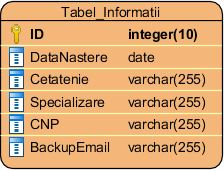
\includegraphics[scale=0.7]{Source/Informatii} 
		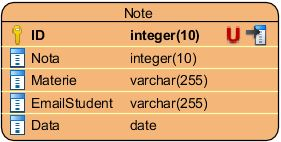
\includegraphics[scale=0.8]{Source/Note}
		\begin{figure}[!h]
			{\caption*{Modelul tabelelor Informații și Note.}}
		\end{figure}
	\end{center}

	Tabelul Note se va folosi de cheia primară ( ID ) în cazul se va face o introducere a două note separate, dar, care sunt la fel. 

		\subsubsection*{Crearea bazei de date}
	
		Prin folosirea librariilor SQLiteDatabase [\ref{SQLiteDatabase}] și SQLiteOpenHelper [\ref{SQLiteOpenHelper}], se va incerca crearea bazei de date la fiecare pornire a aplicatiei. Prin aceasta metoda, in cazul in care baza de date a fost manual stearsa din fisierele telefonului mobil sau o eroare s-a intamplat care a dus la coruperea bazei de date, baza de date va fi recreata. 

	\begin{verbatim}
    public void onCreate(SQLiteDatabase db) {

        String CreateTableInformatii = "CREATE TABLE IF NOT EXISTS " + Table_Informatii + 
              " ( ID INTEGER PRIMARY KEY AUTOINCREMENT, " + DataNastere + " TEXT, " + 
              Cetatenie + " TEXT, " + CNP + " TEXT, " + BackupEmail + " TEXT, " + Specializare + 
              " TEXT)";

        String CreateTableNote = "CREATE TABLE IF NOT EXISTS " + Table_Note + 
              " (ID INTEGER PRIMARY KEY AUTOINCREMENT, " +
                Nota + " TEXT, " + Materie + " TEXT, " + Data + " TEXT, " + Semestru + " TEXT)";

        db.execSQL(CreateTableInformatii);
        db.execSQL(CreateTableNote);
    }
	\end{verbatim}
	
		\subsubsection*{Introducerea datelor in baza de date.}

	Informațiile preluate de la transferul de date dintre server și aplicația mobilă vor fi introduse în baza de date, în tabelele Informații și Note. Deoarece toate datele trimise de la server sunt trimise într-un singur mesaj, aceastea, odată la ajungerea lor la aplicație, trebuie despărțite. \\

	Prima parte a mesajului va consta în datele studentului. Aceste date vor veni în formatul următor:\\

	\textbf{Dată Naștere, Cetățenie, CNP, BackupEmail, Specializare} \\

	 După ce aceste date vor ajunge la aplicație, acestea vor fi inserate în baza de date și pregătite pentru a afișa utilizatorului aplicației informațiile cerute.

	\begin{verbatim}
    SQLiteDatabase database = this.getWritableDatabase();
    ContentValues contentValues = new ContentValues();

    String[] TabelData = Details.split(":");

    contentValues.put(DataNastere, TabelData[0]);
    contentValues.put(Cetatenie, TabelData[1]);
    contentValues.put(CNP, TabelData[2]);
    contentValues.put(BackupEmail, TabelData[3]);
    contentValues.put(Specializare, TabelData[4]);

    Log.d("Database Informative: ", "datele urmatoare: " + Details + 
        " sunt adaugate in " + Table_Informatii);

    long result = database.insert(Table_Informatii, null, contentValues);
	\end{verbatim}

	Fiecare acțiune realizată de către aplicație care are o orice legătură cu baza de date va fi pusă într-un jurnal local al aplicației numit \textbf{Database Informative}.

	Cea de a doua parte a mesajului va consta în notele studentului. Această parte de mesaj are posibilitatea de a fi goală (în cazul în care, spre exemplu, utilizatorul tocmai a fost înregistrat în baza de date). Această parte a mesajului va veni în felul următor. \\

	\textbf{Nota, Materia, Data, Semestrul, ":"} \\

	Caracterul special ":" va fi folosit pentru a despărți notele în cazul în care sunt mai mult de cât una. În acest caz, formatul de mai sus va fi repetat de câte ori este nevoie pentru a transmite datele de la server la client. Acest lucru nu va face ca mesajul trimis de către server să fie despărțit în mai multe mesaje, el rămânând tot la unul singur.

	Dupa ce aceste date vor ajunge la aplicatie, acestea vor fi inserate in baza de date si pregatite (daca este cazul) pentru a afisa utllizatorului aplicatiei informatiile cerute.

	\begin{verbatim}
    SQLiteDatabase database = this.getWritableDatabase();
    ContentValues contentValues = new ContentValues();

    String[] TabelNote = Details.split("~");

    for (String parse : TabelNote) {
        String[] Note = parse.split(":");
        String Nota = Note[0];
        String Materie = Note[1];
        String Data = Note[2];
        String Semestru = Note[3];

    contentValues.put(DataBase.Nota, Nota);
    contentValues.put(DataBase.Materie, Materie);
    contentValues.put(DataBase.Data, Data);
    contentValues.put(DataBase.Semestru, Semestru);

    Log.d("DataBase Informative", "datele urmatoare: " + parse + " sunt adaugate in " + Table_Note);

    long result = database.insert(Table_Note, null, contentValues);

	\end{verbatim}
		\subsubsection*{Actualizarea bazei de date.}

	 Actualizarea bazei de date se va întâmplă de fiecare dată când utilizatorul se va re-conecta la server de pe acelasi dispozitiv mobil. Acest lucru trebuie făcut din următoarele două motive:
	\begin{itemize}
		\item În cazul în care un alt utilizator dorește să-și acceseze contul său de pe alt dispozitiv mobil care are deja o logare validă de pe alt cont.
		\item Pentru a nu se umple baza de date cu date repetitive (precum notele).
	\end{itemize}

	La fiecare conexiune in care serverul NU va trimite un mesaj de eroare inapoi, aplicatia mobila va sterge toate informatiile din cele doua tabele si le va actualiza cu noile date primite de la server prin utilizarea funcției \textbf{UpdateData}.

	\begin{verbatim}
    public void UpdataData()
    {
        SQLiteDatabase database = this.getWritableDatabase();
        String UpdateInformatii = "DELETE FROM " + Table_Informatii;
        String UpdateNote = "DELETE FROM " + Table_Note;

        database.execSQL(UpdateInformatii);
        database.execSQL(UpdateNote);
    }
	\end{verbatim}
	
	\newpage

	\section{Prezentarea Aplicației UVT Student App}

		Aplicația mobilă UVT Student APP constă în trei activități. Dintre aceste trei activități, două dintre ele vor putea fi accesate doar după ce baza de date locală a aplicației va conține date. Cea de a treia activitate a aplicației va constă în activitatea pe care utilizatorul o va vedea la pornirea aplicației, și anume, activitatea prin care utilizatorul va completa acțiunea de Login. \\

		Activitatea de afișare a informațiilor și activitatea de afișare a notelor sunt două activități legate, create sub formă unei activități de tipul \textbf{Bottom navigation activity}. Această activitate va permite interschimbarea dintre cele două activități într-un mod ușor pentru utilizator. Activitatea va avea două butoane pentru a prezenta activitatea curentă pe care utilizatorul se află în momentul respectiv. Aceste butoane vor prezenta activitatea curentă având denumirile "Detalii personale", respectiv, "Note". Aceste două activități, după ce cel puțin o conexiune validă cu serverul a fost realizată, pot fi accesate fără că o logare să fie necesară.

		\subsection{Activitatea de Logare}

		Activitatea de Logare este activitatea principală a aplicației. Această activitate ne va prezența cu funcționalitățile principale ale aplicației::
		\begin{itemize}
			\item Login
			\item Vizualizare date
		\end{itemize}

		În imaginea următoare, se poate observa interfața activității de logare.

	\begin{center}
		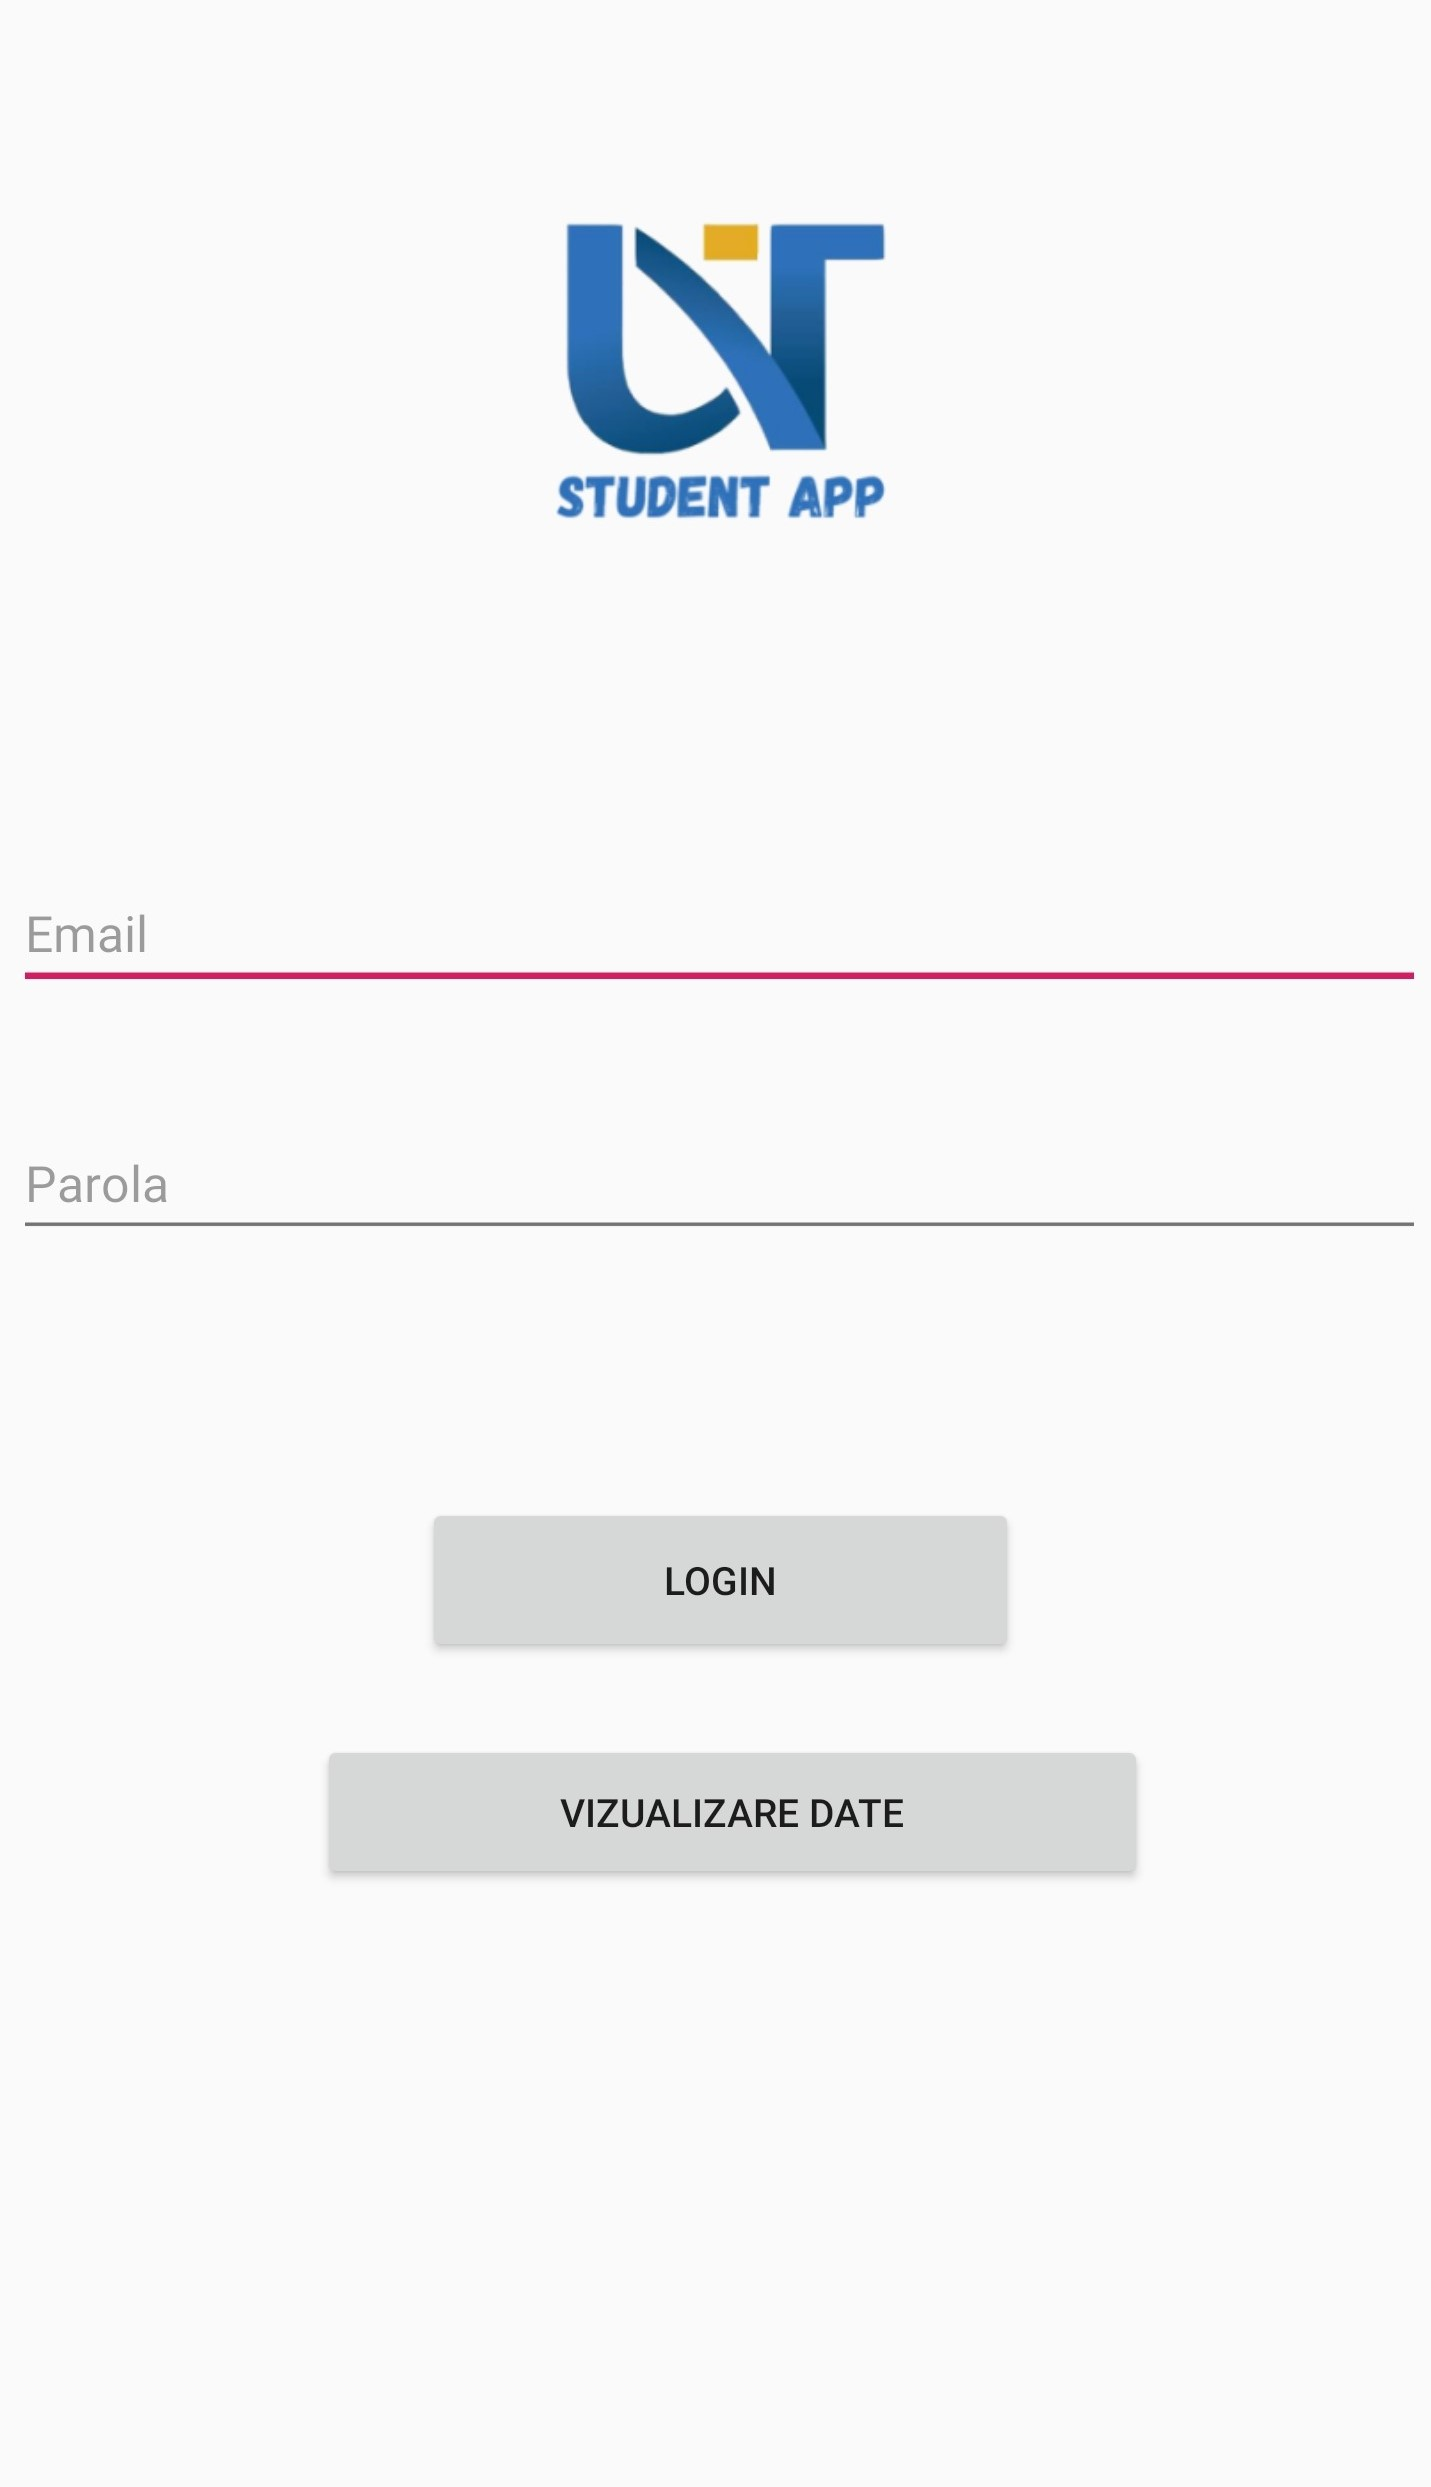
\includegraphics[scale=0.15]{Source/UVTMain}
		\begin{figure}[!h]
			{\caption*{Interfața Activități principale de Logare.}}
		\end{figure}
	\end{center}

		\subsubsection*{Login}
		Pentru folosirea funcționalității de Login, utilizatorul va trebui, mai întâi, să introducă un Email și o Parolă validă (validitatea datelor a fost explicată aici [\ref{Credentiale}].

		După ce un Login valid va fi detectat, activitatea de "Afișare a informațiilor" va fi automat deschisă cu informațiile primite de la baza de date.

		\subsection{Activitatea de afișare a informațiilor}

		  Activitatea de afișare a informațiilor va fi activitatea unde, utilizatorul aplicației, va putea să-și vadă datele personale. În această activitate, vor fi afișare următoarele informații:
	\begin{itemize}
		\item Dată Naștere
		\item Cetățenie
		\item Specializare
		\item CNP
		\item BackupEmail
	\end{itemize}

		În imaginea următoare, se poate observa interfață activității de afișare a informațiilor. 

	\begin{center}
		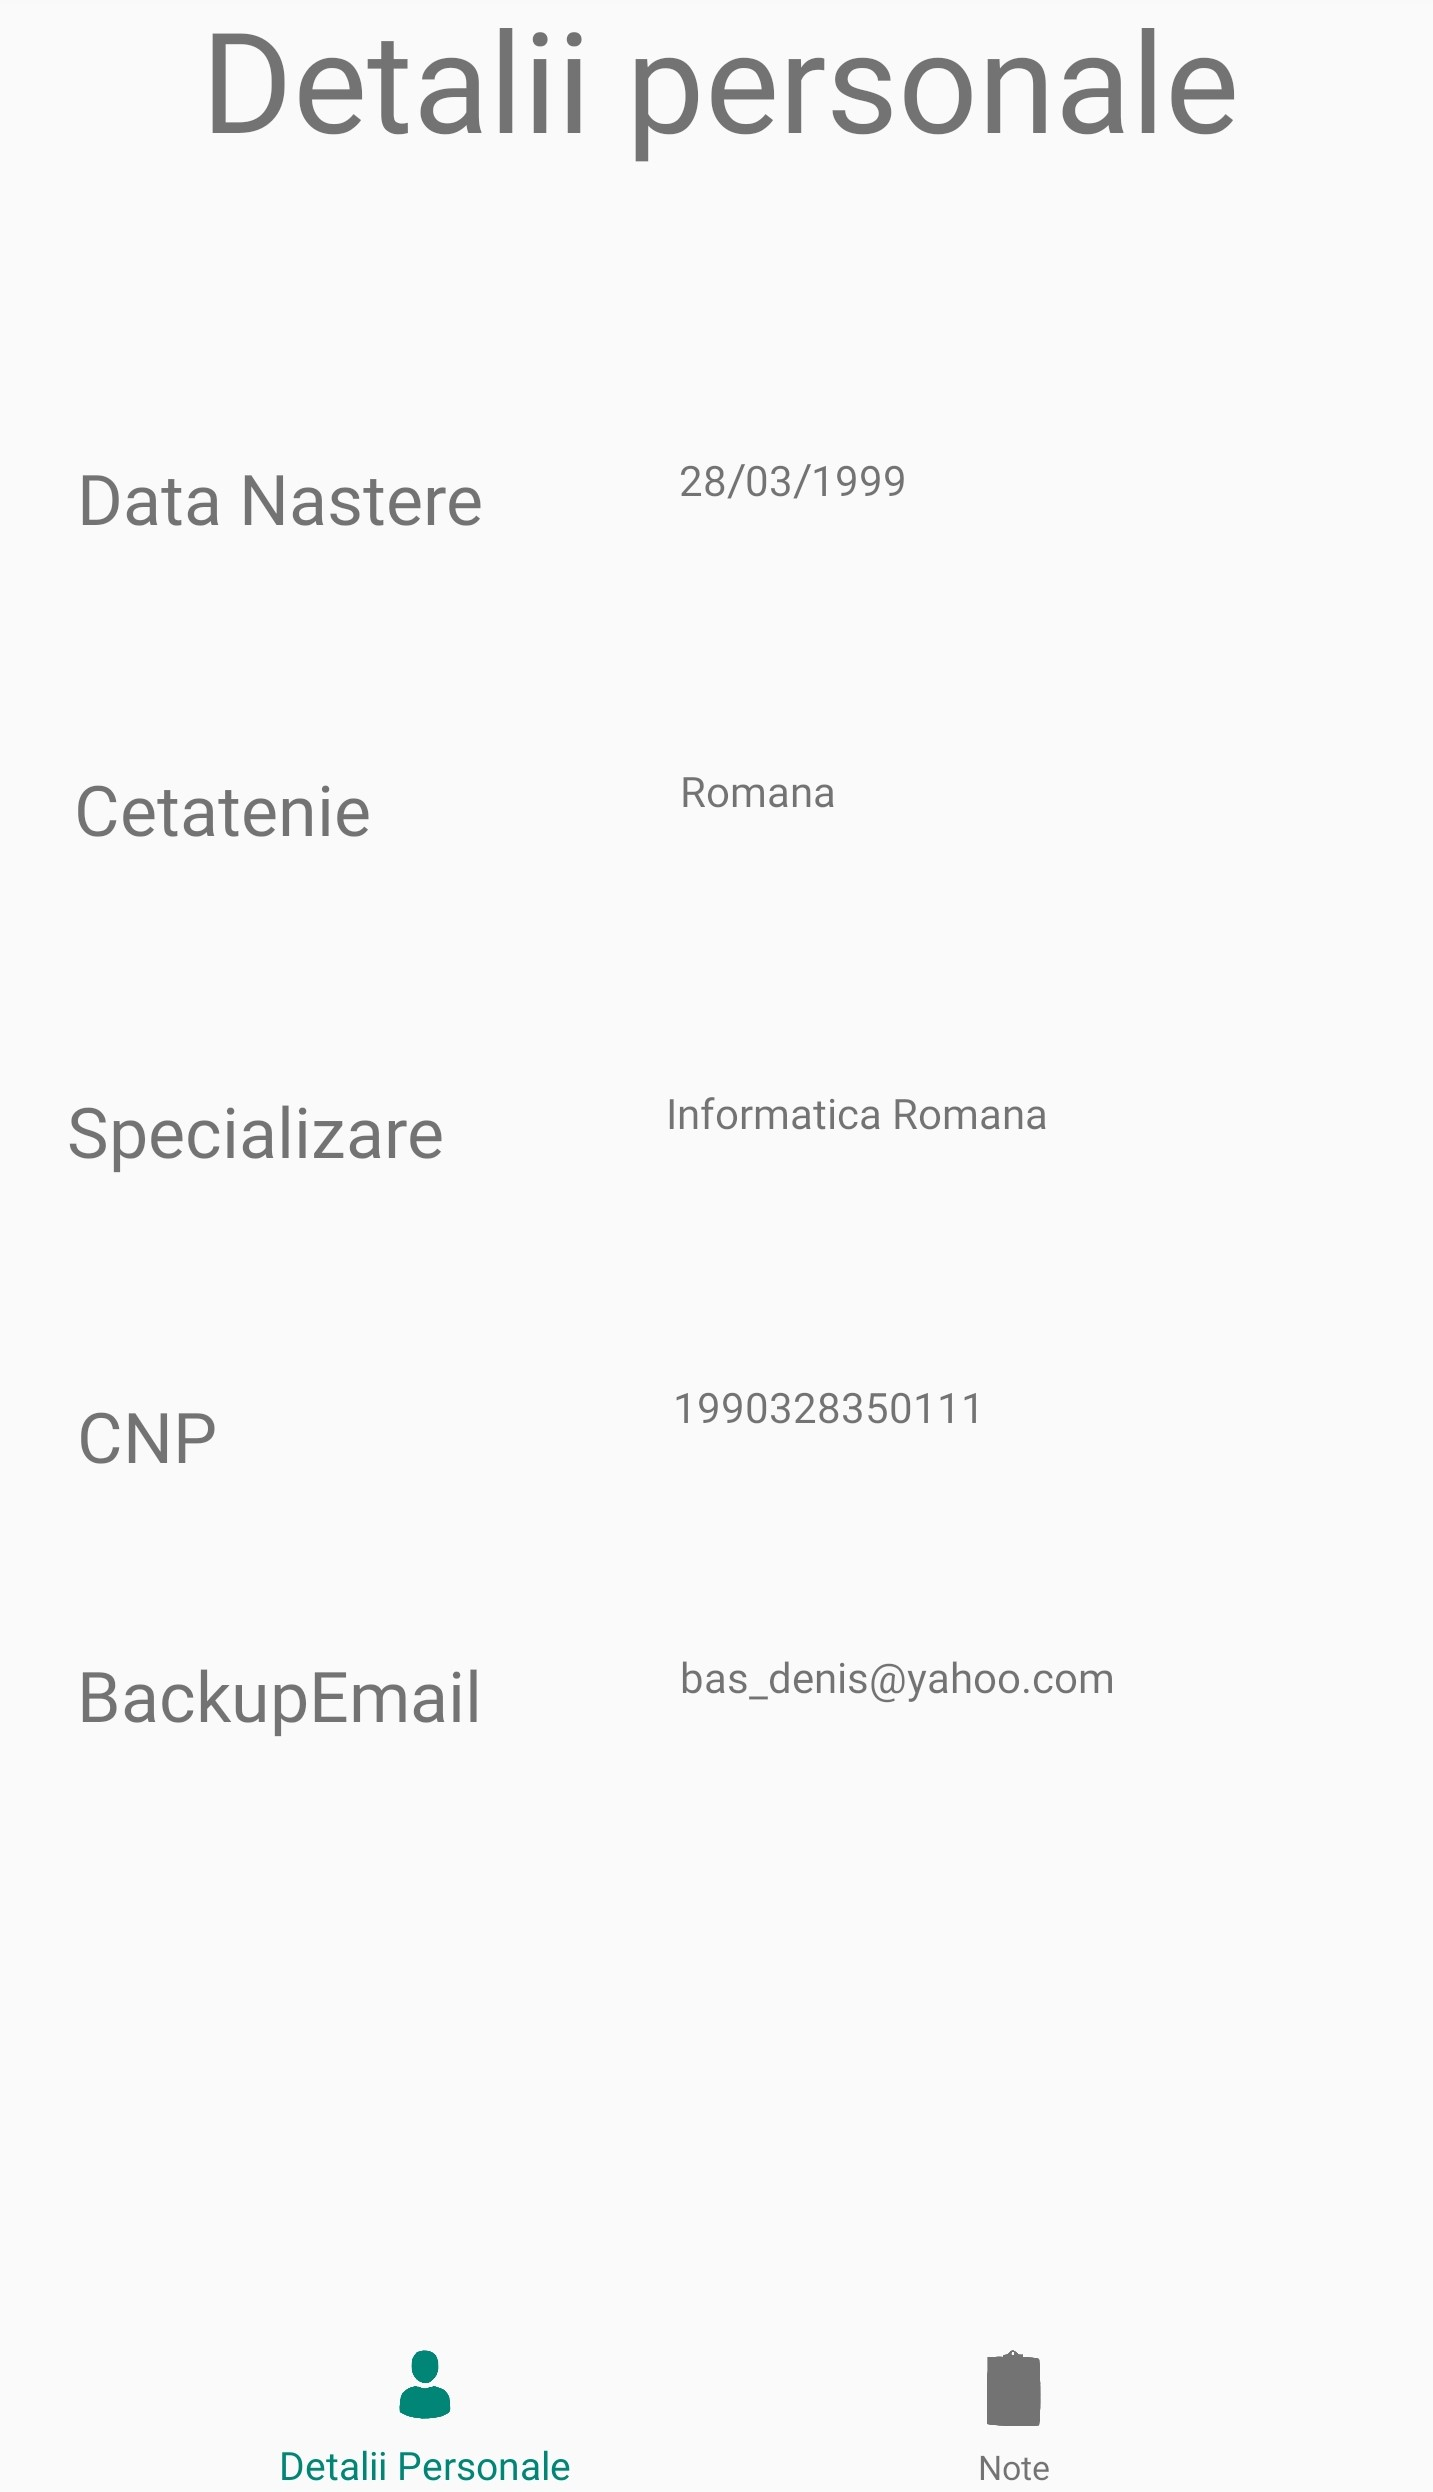
\includegraphics[scale=0.15]{Source/UVTDetalii}
		\begin{figure}[!h]
			{\caption*{Interfața Activități de Detalii.}}
		\end{figure}
	\end{center}

		\subsection{Activitatea de afișare a notelor}

		Activitatea de afisare a notelor va fi activitatea unde, utilizatorul aplicatiei, va putea sa-si vada notele personale de la facultate. In aceasta activitate, se va prezenta utilizatorului o lista cu notele pe care acesta le are. Formatul acestei liste va fi de tipul urmator:
	\begin{itemize}
		\item Materie
		\item Nota
		\item Data
		\item Semestrul
	\end{itemize}
	
		Dupa ce baza de date a fost actualizata la o logare valida, tabelul de Note are posibilitatea de a ramane gol, acest lucru fiind posibil in cazul in care studentul este inregistrat recent in baza de date. In cazul in care tabelul Note NU este gol, datele vor fi afisare in activitatea de afisare a notelor, ordonate in functie de semestru. \\

		În imaginea următoare, se poate observa interfață activității de afișare a notelor. 

	\begin{center}
		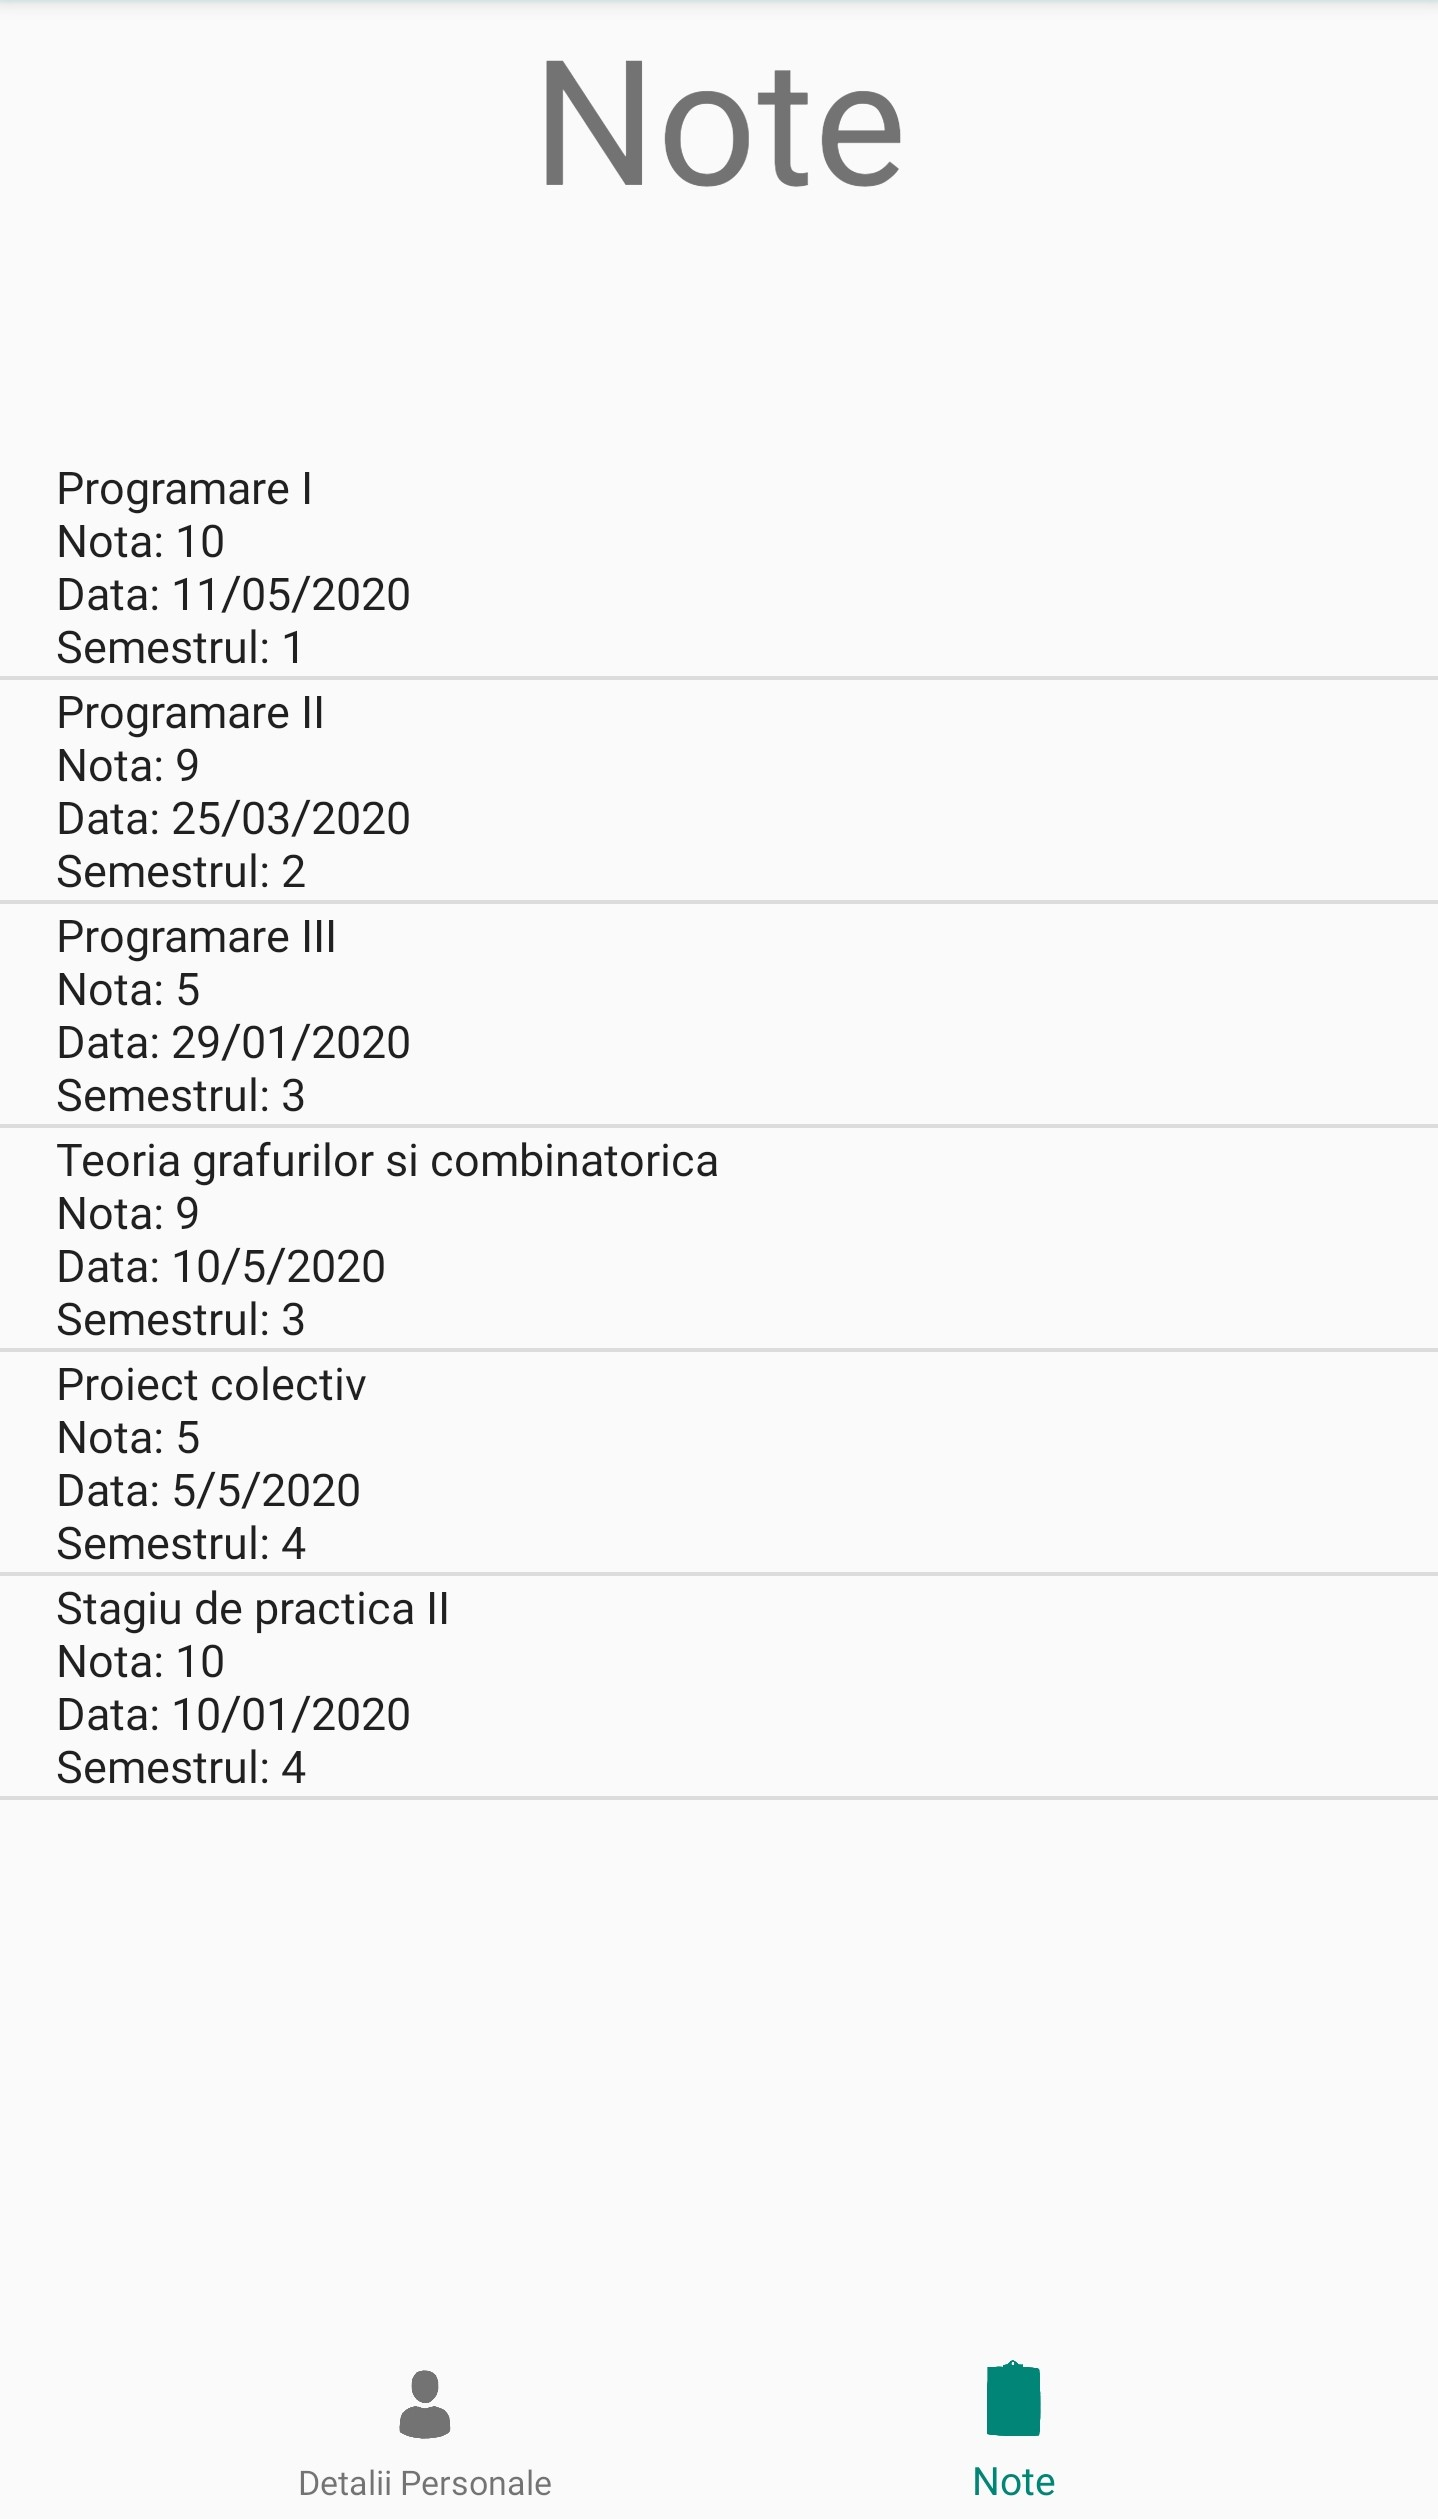
\includegraphics[scale=0.15]{Source/UVTNote}
		\begin{figure}[!h]
			{\caption*{Interfața Activități de Note.}}
		\end{figure}
	\end{center}

	\newpage
	\section{Aplicații asemănătoare deja existente}

	 Aplicații deja asemănătoare aplicației UVT Student App ( aplicației mobile, nu serverul ) sunt:
	\begin{itemize}
		\item Site-ul \url{https://studentweb.uvt.ro/}.
			Acest site are ideea principală asemenatoare cu aplicația UVT Student App, dar, abordarea funcționalităților și menținerea serverului sunt diferite.
		\item Aplicații facultative informative (ex. Site-uri/Aplicații telefonice create/menținute de cadre facultative)
	\end{itemize}

	\newpage
	\section{Concluzii si directii viitoare}

	În concluzie, aplicația UVT Student App și serverul creat pentru suportarea acestei aplicații și-au atins scopul de a crea un mediu ușor de accesat, puțin costisitor și care să ofere studentului o modalitate de a-și accesa notele sale într-un mediu offline. 

 Direcțiile viitoare ale aplicației vor fi prin adăugarea unor funcționalități noi, dar, nu s-au putut realiza din prima din cauza lipsei de informații:
	\begin{itemize}
		\item Funcționalitate de a cere o parolă nouă în cazul în care, utilizatorul aplicației, va avea nevoie de o resetare a parolei.
		\item Crearea unei versiuni a aplicației pentru profesori.
		\item Anunțarea utilizatorului, prin email, în cazul în care o notă este adăugată/modificată.
	\end{itemize}

	\newpage
	\section{Bibliografie} \label{Bibliografie}
	
	\vspace{1cm}

		BCryptPasswordEncoder: \url{https://docs.spring.io/spring-security/site/docs/current/api/org/springframework/
security/crypto/bcrypt/BCryptPasswordEncoder.html}\label{PasswordEncoder}\\ \\
		Java SMTP: \url{https://www.javatpoint.com/simple-mail-transfer-protocol} \label{SMTP}
		SQLite: \url{https://docs.oracle.com/javase/8/docs/api/index.html?java/sql/package-summary.html}\label{SQL} \\ \\
		Connectivity Manager: \url{https://developer.android.com/reference/android/net/ConnectivityManager}\label{ConnMan} \\ \\
		SQLiteDatabase : \url{https://developer.android.com/reference/android/database/sqlite/SQLiteDatabase}\label{SQLiteDatabase} \\ \\
		SQLiteOpenHelper: \url{https://developer.android.com/reference/android/database/sqlite/SQLiteOpenHelper}\label{SQLiteOpenHelper}
		

\end{document}